\chapter{Semantic Metalogic Redux} \label{ch:sem2}

%% TO DO: semantics for many-sorted logic, but use M(-) instead of
%% ...

In the previous chapter, we covered some of the standard topics in
model theory --- focusing on those parts we think are of most interest
to philosophers.  However, the semantic methods of the previous
chapter are restricted to the special case of single-sorted logic.  In
this chapter, we cover semantics for many-sorted logic.  But our aim
here is not many-sorted logic for its own sake.  Indeed, we feel that
one first really understands single-sorted logic when one sees it as a
special case of many-sorted logic.  What's more, even for
single-sorted theories, some of the most interesting relations between
theories can only be explicated by means of many-sorted methods.

\section{Structures and models}

For the most part, generalizing semantics to many-sorted logic is
straightforward: where a single-sorted structure $M$ has a single
domain set, a many-sorted structure has a separate domain set
$M(\sigma )$ for each separate sort symbol $\sigma\in \Sigma$.
Moreover, if a $\Sigma$-formula $\phi$ has free variables of different
sorts, then its extension $M(\phi )$ will be a subset of a Cartesian
product of different domains.

\begin{defn} Let $\Sigma$ be a signature.  A
  \emph{$\Sigma$-structure} $M$ is a mapping from $\Sigma$ to
  appropriate structures in the category $\cat{Sets}$.  In particular:
  \begin{itemize}
  \item $M$ maps each sort symbol $\sigma \in \Sigma$ to a set
    $M(\sigma )$.
  \item $M$ maps each $n$-ary relation symbol $p$ of sort
    $\sigma _1\times\cdots \times \sigma _n$ to a subset
    $M(p)\subseteq M(\sigma _1)\times\cdots\times M(\sigma _n)$.
  \item $M$ maps each function symbol $f$ of sort
    $\sigma _1\times\cdots\times \sigma _n\to \sigma _{n+1}$ to a
    function
    $M(f):M(\sigma _1)\times \cdots \times M(\sigma _n)\to M(\sigma
    _{n+1})$.
  \end{itemize}
\end{defn}

As was the case with single-sorted logic, each $\Sigma$-structure
$M$ extends to a map, still called $M$, from $\Sigma$-terms to
functions, and from $\Sigma$-formulas to subsets.  In particular:
\begin{itemize}
\item For each term $t$ of type $\sigma _1\times\cdots\times\sigma
    _n\to \sigma _{n+1}$,
    \[ M(t):M_1\times\cdots\times M_n\to M_{n+1} . \]
  \item For each formula $\phi$ of type
    $\sigma _1\times\cdots\times \sigma _n$,
    \[ M(\phi )\: \subseteq \: M_1\times\cdots \times M_n
      .\]
  \end{itemize}

  \begin{defn} Let $M$ and $N$ be $\Sigma$-structures, where $\Sigma$
    has sorts $\sigma _1,\dots ,\sigma _n$.  An \emph{elementary
      embedding} $h:M\to N$ consists of a family
    $\{ h_i \mid \sigma _i \in \Sigma \}$ of functions
    $h_i :M(\sigma _i)\to N(\sigma _i)$ that preserves the extension
    of each $\Sigma$-formula $\phi$.  \label{eeman} \end{defn}

  It's easy to see that the composition of elementary embeddings is an
  elementary embedding.  Thus, for a given theory $T$, we let
  $\mathrm{Mod}(T)$ be the category whose objects are models of $T$
  and whose arrows are elementary embeddings.  Notice that this
  definition directly generalizes the definition we gave for
  single-sorted theories; hence, for a single-sorted theory $T$, there
  is no ambiguity when we write $\mathrm{Mod}(T)$.

%% explain about canonical contexts, and how now the sort of the
%% variable matters too

%% completeness, compactness, Lowenheim-Skolem, Beth

%% we already know that for each many sorted theory T, there is a
%% single-sorted theory T' such that T and T' are Morita equivalent.

%% [[TO DO: can we prove C,C,LS,B for many-valued by reduction to
%% single valued.  For this we need the following results:

%% Now suppose that $T\vDash \phi$.  Then $T'\vDash F\phi$.  By
%% completeness for single-sorted, $T'\vdash F\phi$.  By
%% conservativity of $F$, $T\vdash \phi$.


\section{The dual functor to a translation} \label{sec:dual}

Intuitively speaking, a translation $F:T\to T'$ should induce a
functor $F^*:\mathrm{Mod}(T')\to \mathrm{Mod}(T)$ going in the
opposite direction.  To see this, recall that models of a theory $T'$
aren't static structures, but are more like functors from $T'$ into
the category $\cat{Sets}$.  If we think of a model of $T'$ as a
functor $M:T'\to \cat{Sets}$, then we can precompose this functor with
a translation $F:T\to T'$, giving a functor
\[ T\:\stackrel{F}{\longmapsto} \:T' \:\stackrel{M}{\longmapsto}
  \:\cat{Sets} ,\] i.e.\ we get a model $F^*M=M\circ F$ of $T$.
However, since $M$ and $F$ are not actually functors, we have have to
do some work to validate this intuition.

\begin{defn} Let $F:T\to T'$ be a fixed translation.  Given an
  arbitrary model $M$ of $T'$, we define a $\Sigma$-structure $F^*M$
  as follows:
\begin{itemize}
\item For a sort symbol $\sigma$ of $\Sigma$, first consider the set
  \[ M(F(\sigma )) = M(F(\sigma )_1)\times\cdots\times M(F(\sigma )_n)
    ,\] and its subset $M(D_\sigma )$, where $D_\sigma$ is any one of
  the domain formulas that $F$ associates with $\sigma$.  (These
  domain formulas are all equivalent.)  Since $F$ is a translation,
  and $M$ is a model of $T'$, $M(E_\sigma )$ is an equivalence
  relation on $M(D_\sigma )$.  Let $q:M(D_\sigma )\to Y$ be the
  corresponding quotient map, and let $(F^*M)(\sigma )=Y$.
\item For a relation symbol $p:\sigma _1,\dots, \sigma _n$ of
  $\Sigma$, we define
  \[ (F^*M)(p) \:=\: (q_1\times\cdots\times q_n)(M(Fp)) ,\] where
  $q_i:M(D_{\sigma _i})\to Y_i$ is the corresponding projection.
\item For a function symbol $f:\sigma _1,\dots ,\sigma _n\to \sigma _{n+1}$
  of $\Sigma$, we define $(F^*M)(f)$ be the function with graph
  \[ (q_1\times\cdots\times q_n\times
    q_{n+1})(M(Ff)) .\]
\end{itemize} \end{defn}


%% to do: we want to show that this gives a model functor.  First
%% thing, we want to show that $F^*M$ is a model of $T$.

\begin{note} \label{compat} Suppose that $F:T\to T'$ is a translation,
  and let $\phi (x)$ be a $\Sigma$-formula.  Then $F(\phi )(\vec{x})$
  is compatible with the relation $E(\vec{x},\vec{y})$ in the
  following sense: $T'$ implies that if $F(\phi )(\vec{x})$ and
  $E(\vec{x},\vec{y})$, then $F(\phi )(\vec{y})$.  It follows from
  this that in any model $M$ of $T'$, the subset
  $A\equiv M(F(\phi )(\vec{x}))$ of $M(D)$ is compatible with the
  equivalence relation $M(E(\vec{x},\vec{y}))$.  That is, if
  $q:M(D)\to Y$ is the quotient map induced by
  $M(E(\vec{x},\vec{y}))$, then $q^{-1}(q(A))=A$.  \end{note}

\begin{prop} Suppose that $F:T\to T'$ is a translation, and that
  $\phi$ is a $\Sigma$-formula.  Then $(F^*M)(\phi )$ is the image of
  $M(F(\phi ))$ under the corresponding quotient map $q$. \end{prop}

\begin{proof} To be precise, we prove that the result holds for each
  $\Sigma$-formula $\phi$, and context $x_1,\dots ,x_n$ for $\phi$.
  Once a context $x_1,\dots ,x_n$ for $\phi$ is fixed, we also fix the
  corresponding context $\vec{x}_1,\dots ,\vec{x}_n$ for $F(\phi )$.
  Moreover, for a $\Sigma$-structure $N$, we take $N(\phi )$ to
  mean the extension of $\phi$ relative to the context
  $x_1,\dots ,x_n$.
  
  The base case follows immediately from the definition of $F^*M$.  As
  for inductive cases, we will treat $\wedge$ and $\exists y$, and
  leave the others to the reader.  We simplify notation as follows:
  let $N=F^*M$, and for each $\Sigma$-formula $\phi$, let
  $\phi ^*=F(\phi )$.  \begin{itemize}
  \item Suppose that the result is true for $\phi _1$ and $\phi _2$,
    in any of their contexts.  Let $x_1,\dots ,x_n$ be a context for
    $\phi _1\wedge\phi _2$, hence also for $\phi _1$ and $\phi _2$.
    Let $D=D(\vec{x}_1)\wedge\cdots\wedge D(\vec{x}_n)$ be the
    conjunction of domain formulas for $x_1,\dots ,x_n$; let
    $E=E(\vec{x}_1,\vec{y}_1)\wedge\cdots\wedge
    E(\vec{x}_n,\vec{y}_n)$ be the conjunction of the corresponding
    equivalence relations; and let $q:M(D)\to Y$ be the quotient map
    determined by $M(E)$.  If we let $A_i=M(\phi _i^*)\subseteq M(D)$,
    then the inductive hypothesis asserts that $N(\phi _i)=q(A_i)$.
    Since $(\phi _1\wedge \phi _2)^*=\phi _1^*\wedge \phi _2^*$, it
    follows that $M((\phi _1\wedge\phi _2)^*)=A_1\cap A_2$.  Thus,
    \[ \begin{array}{l l l} q(M(\phi ^*)) & =& q(A_1\cap A_2) \\
      &= & q(A_1)\cap q(A_2) \\
      & = & N(\phi _1)\cap N(\phi _2) \\
      & = & N(\phi ) .\end{array} \]
The second equation follows from the note above; the third equation
follows from the induction hypothesis; and the final equation  by the fact that
$N$ is a $\Sigma$-structure.  

\item Suppose that the result is true for $\phi$.  That is,
  \[ N(\phi ) \: = \: (q_1\times q_2)(M(\phi ^*)) ,\] where
  $q_1:M(D_1)\to Y_1$ and $q_2:M(D_2)\to Y_2$ are the quotient maps.
  We show that the result is also true for $\exists y\phi$.  Consider
  the commuting diagram:
  \[ \begin{tikzcd}
      M(D_1)\times M(D_2) \arrow{r}{\pi} \arrow{d}{q_1\times q_2} & M(D_2) \arrow{d}{q_2}  \\
      Y_1\times Y_2 \arrow{r}{\pi} & Y_2 \end{tikzcd} \] where $\pi$
  is the projection onto the second coordinate.  By definition,
  \[ M((\exists y\phi )^*)=M(\exists \vec{y}(\phi ^*))=\pi ^*(M(\phi
    ^*)) .\] Hence, 
  \[ \begin{array}{l l l} N(\exists y\phi ) & =\pi (N(\phi ))= \pi
                                              ((q_1\times q_2)(M(\phi
                                              ^*))) \\
       & = q_2(\pi ^*(M(\phi ^*))) = q_2(M((\exists y\phi )^*))
         . \end{array} \] Thus, the result also holds for $\exists
     y\phi$. 
  \end{itemize}
\end{proof}

\begin{prop} Let $F:T\to T'$ be a translation.  If $M$ is a model of
  $T'$, then $F^*M$ is a model of $T$. \end{prop}

\begin{proof} Let $\phi$ be a $\Sigma$-formula in context
  $x_1,\dots ,x_n$ such that $T\vdash\phi$.  Since $F:T\to T'$ is a
  translation, $T'\vdash F(\phi )$.  If $M$ is a model of $T'$, then 
  \[ M(F(\phi )) \: = \: M(\vec{x}_1,\dots ,\vec{x}_n) .\] By the
  previous proposition, $(F^*M)(\phi )$ is the image of $M(F(\phi ))$
  under the quotient map $q:M(D(\vec{x}_1,\dots ,\vec{x}_n))\to Y$
  induced by the equivalence relation $M(E)$, where
  \[ E \: = \: E(\vec{x}_1,\vec{y}_1)\wedge\cdots\wedge
    E(\vec{x}_n,\vec{y}_n) .\] Thus,
  $(F^*M)(\phi )=Y=(F^*M)(x_1,\dots ,x_n)$, and $F^*M$ is a model of
  $T$.  \end{proof}

Thus, if $F:T\to T'$ is a translation, then $F$ gives rise to a
mapping $F^*$ from the objects of $\mathrm{Mod}(T')$ to the objects of
$\mathrm{Mod}(T)$.  We now define $F^*$ on the arrows of
$\mathrm{Mod}(T')$.  Let $M$ and $N$ be models of $T'$, and let
$h:M\to N$ be an elementary embedding.  Recall that $h$ consists of
family $\{ h_\sigma \mid \sigma \in \Sigma '\}$ of functions
$h_i :M(\sigma )\to N(\sigma )$ that preserves the extension of each
$\Sigma '$-formula $\psi$.  Now let $\sigma$ be a sort of $\Sigma$,
and let $\vec{x}$ be a sequence of $\Sigma '$-variables of sort
$F(\sigma )=\sigma _1,\dots ,\sigma _n$.  Consider the following
diagram:
\[ \begin{tikzcd} M(D_\sigma ) \arrow{r}{h} \arrow{d}{q_M} &
    N(D_\sigma )
    \arrow{d}{q_N} \\
    (F^*M)(\sigma )\arrow[dashed]{r}{F^*h} & (F^*N)(\sigma
    ) \end{tikzcd} \] where $q_M$ and $q_N$ are the quotient maps
induced by $M(E)$ and $N(E)$ respectively, and $h$ is the restriction
of $h_1\times\cdots\times h_n$ to $M(D_\sigma )$, which is
well-defined since $h$ preserves the extensions of
$\Sigma '$-formulas.  Moreover, if
$\langle \vec{a},\vec{b}\rangle\in M(E)$, then
$\langle h(\vec{a}),h(\vec{b})\rangle \in N(E)$.  Thus, $h$ determines
a unique function $F^*h:(F^*M)_\sigma \to (F^*N)_\sigma $ such that
the above diagram commutes.

  Now let $\phi$ be a $\Sigma$-formula.  Then $a\in (F^*M)(\phi )$ iff
  $a=q_M(b)$, for some $b\in M(F(\phi ))$.  Moreover,
  $b\in M(F(\phi ))$ iff $h(b)\in N(F(\phi ))$ iff
  $q_N(h(b))\in (F^*N)(\phi )$.  This shows that $a\in (F^*M)(\phi )$
  iff $(F^*h)(a)\in (F^*N)(\phi )$.  Therefore, $F^*h$ is an
  elementary embedding.

It is easy to see that $F^*$ preserves composition of elementary
  embeddings, as well as identity morphisms of models.  Therefore
  $F^*$ is a functor from $\mathrm{Mod}(T')$ to $\mathrm{Mod}(T)$.


  \begin{disc} It is tempting to think that any functor
    $G:\mathrm{Mod}(T')\to \mathrm{Mod}(T)$ corresponds to some
    potentially interesting relationship between the theories $T$ and
    $T'$.  However, functors of the form
    $F^*:\mathrm{Mod}(T')\to\mathrm{Mod}(T)$, where $F:T\to T'$ is a
    translation, seem to be singled out by the fact that they preserve
    important theoretical structures.  First, the functor $F^*$ is
    ``definable'' in the sense that the resulting model $F^*M$ is
    defined in terms of the model $M$, and in a uniform fashion.  That
    is, the ``same definition'' of the new model works, regardless of
    which model we plug into $F^*$.  (For more on the notion of
    definable functors, see \cite{hudetz-new}.)  Second, in the case
    of propositional theories, a functor
    $G:\mathrm{Mod}(T')\to \mathrm{Mod}(T)$ is simply a function from
    the Stone space $X'$ of $T'$ to the Stone space $X$ of $T$; and
    functors of the form $F^*$ are precisely the continuous
    functions.  \end{disc}

  We now have the tools we need to do some work with the notion of
  Morita equivalence.  We'll first show how similar Morita equivalence
  is to its poorer cousin, definitional equivalence.  In particular,
  we'll show that Morita equivalent theories have equivalent
  categories of models.

\section{Morita equivalence implies categorical equivalence} \label{sec:moca}

As with a definitional extension, a Morita extension $T^+$ should
``say nothing more'' than the original theory $T$.  We will make this
idea precise by proving three results about the relationship between
$\mathrm{Mod}(T^+)$ and $\mathrm{Mod}(T)$.  First, the models of $T^+$
are ``determined'' by the models of $T$.

\begin{thm}[Barrett] Let $\Sigma\subseteq\Sigma^+$ be signatures and
  $T$ a $\Sigma$-theory. If $T^+$ is a Morita extension of $T$ to
  $\Sigma^+$, then every model $M$ of $T$ has a unique expansion (up
  to isomorphism) $M^+$ that is a model of $T^+$. \label{mor1}
\end{thm}

Before proving this result, we introduce some notation and prove a
lemma.  Suppose that a $\Sigma^+$-theory $T^+$ is a Morita extension
of a $\Sigma$-theory $T$. Let $M$ and $N$ be models of $T^+$ with
$h:M|_\Sigma\rightarrow N|_\Sigma$ an elementary embedding between the
$\Sigma$-structures $M|_\Sigma$ and $N|_\Sigma$. The elementary
embedding $h$ naturally induces a map $h^+:M\rightarrow N$ between the
$\Sigma^+$-structures $M$ and $N$.

We know that $h$ is a family of maps
$h_\sigma: M_\sigma\rightarrow N_\sigma$ for each sort
$\sigma\in\Sigma$.  (Here we have used $M_\sigma$ for the domain
$M(\sigma )$ that $M$ assigns to the sort symbol $\sigma$, and
similarly for $N_\sigma$.)  In order to describe $h^+$ we need to
describe the map $h^+_\sigma:M_\sigma\rightarrow N_\sigma$ for each
sort $\sigma\in\Sigma^+$. If $\sigma\in\Sigma$, we simply let
$h_\sigma^+=h_\sigma$.  On the other hand, when
$\sigma\in\Sigma^+\backslash\Sigma$, there are four cases to consider.
We describe $h^+_\sigma$ in the cases where the theory $T^+$ defines
$\sigma$ as a product sort or a subsort. The coproduct and quotient
sort cases are described analogously.

First, suppose that $T^+$ defines $\sigma$ as a product sort. Let
$\pi_1,\pi_2\in\Sigma^+$ be the projections of arity
$\sigma\rightarrow\sigma_1$ and $\sigma\rightarrow\sigma_2$ with
$\sigma_1,\sigma_2\in\Sigma$. The definition of the function
$h^+_\sigma$ is suggested by the following diagram.
\[ 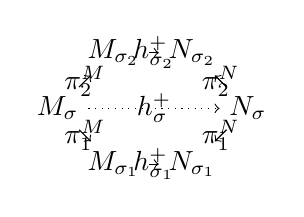
\begin{tikzpicture} 
   \node(1) {$M_\sigma$};
   \node(2) [below right of=1] {$M_{\sigma_1}$};
   \node(3) [right of =2] {$N_{\sigma_1}$};
   \node(4) [above right of=3] {$N_{\sigma}$};
   \node(5) [above right of=1] {$M_{\sigma_2}$};
   \node(6) [right of=5] {$N_{\sigma_2}$};
   \draw[->, dotted] (1) to node {$h^+_\sigma$} (4);
   \draw[->] (1) to node [swap] {$\pi_1^M$} (2);
   \draw[->] (2) to node {$h^+_{\sigma_1}$} (3);
   \draw[->] (4) to node {$\pi_1^N$} (3);
   \draw[->] (1) to node {$\pi_2^M$} (5);
   \draw[->] (5) to node {$h^+_{\sigma_2}$} (6);
   \draw[->] (4) to node [swap] {$\pi_2^N$} (6);
\end{tikzpicture} \] Let $m\in M_\sigma$. We define $h^+_\sigma(m)$ to
be the unique $n\in N_\sigma$ that satisfies both
$\pi_1^N(n)=h^+_{\sigma_1}\circ\pi_1^M(m)$ and
$\pi_2^N(n)=h^+_{\sigma_2}\circ\pi_2^M(m)$. We know that such an $n$
exists and is unique because $N$ is a model of $T^+$ and $T^+$ defines
the symbols $\sigma$, $\pi_1$, and $\pi_2$ to be a product sort. One
can verify that this definition of $h^+_\sigma$ makes the above
diagram commute.
%Using the fact that $h_{\sigma_1}$ and $h_{\sigma_2}$ are injective, one can verify that $h_\sigma$ must be injective too.

Suppose, on the other hand, that $T^+$ defines $\sigma$ as the subsort
of ``elements of sort $\sigma_1$ that are $\phi$.'' Let $i\in\Sigma^+$
be the inclusion map of arity $\sigma\rightarrow\sigma_1$ with
$\sigma_1\in\Sigma$. As above, the definition of $h^+_\sigma$ is
suggested by the following diagram.
\[ 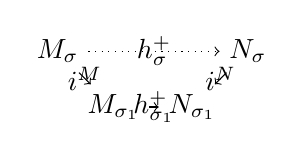
\begin{tikzpicture}
\node(1) {$M_\sigma$};
\node(2) [below right of=1] {$M_{\sigma_1}$};
\node(3) [right of =2] {$N_{\sigma_1}$};
\node(4) [above right of=3] {$N_{\sigma}$};
\draw[->, dotted] (1) to node  {$h^+_\sigma$} (4);
\draw[->] (1) to node [swap] {$i^M$} (2);
\draw[->] (2) to node {$h^+_{\sigma_1}$} (3);
\draw[->] (4) to node {$i^N$} (3);
\end{tikzpicture} \]
Let $m\in M_\sigma$. We see that following implications hold:
\begin{align*}
M\vDash\phi[i^M(m)]&\Rightarrow M|_\Sigma\vDash\phi[i^M(m)]\\
&\Rightarrow N|_\Sigma\vDash\phi[h^+_{\sigma_1}( i^M(m))]\Rightarrow N\vDash\phi[h^+_{\sigma_1}( i^M(m))]
\end{align*}
The first and third implications hold since $\phi(x)$ is a
$\Sigma$-formula, and the second holds because
$h_{\sigma_1}=h^+_{\sigma_1}$ and $h$ is an elementary
embedding. $T^+$ defines the symbols $i$ and $\sigma$ as a subsort and
$M$ is a model of $T^+$, so it must be that $M\vDash \phi[i^M(m)]$. By
the above implications, we see that
$N\vDash\phi[h^+_{\sigma_1}( i^M(m))]$. Since $N$ is also a model of
$T^+$, there is a unique $n\in N_\sigma$ that satisfies
$i^N(n)=h^+_{\sigma_1}(i^M(m))$. We define $h^+_\sigma(m)=n$. This
definition of $h^+_\sigma$ again makes the above diagram commute.

When $T^+$ defines $\sigma$ as a coproduct sort or a quotient sort one
describes the map $h^+_\sigma$ analogously.  We leave it to the reader
to work out the details of these cases.

For the purposes of proving Theorem \ref{mor1}, we need the following
simple lemma about this map $h^+$.

\begin{lemma} If $h:M|_\Sigma\rightarrow N|_\Sigma$ is an isomorphism,
  then $h^+:M\rightarrow N$ is an isomorphism. \label{lemmon}
\end{lemma}

\begin{proof} We know that $h_\sigma:M_\sigma\rightarrow N_\sigma$ is
  a bijection for each $\sigma\in\Sigma$. Using this fact and the
  definition of $h^+$, one can verify that
  $h^+_\sigma:M_\sigma\rightarrow N_\sigma$ is a bijection for each
  sort $\sigma\in\Sigma^+$. So $h^+$ is a family of bijections. And
  furthermore, the commutativity of the above diagrams implies that
  $h^+$ preserves any function
  symbols %$\pi_1,\pi_2, \rho_1,\rho_2, i,$ and $\epsilon$
  that are used to define new sorts.

  It only remains to check that $h^+$ preserves predicates, functions,
  and constants that have arities and sorts in $\Sigma$. Since
  $h:M|_\Sigma\rightarrow N|_\Sigma$ is a isomorphism, we know that
  $h^+$ preserves the symbols in $\Sigma$. So let
  $p\in\Sigma^+-\Sigma$ be a predicate symbol of arity
  $\sigma_1\times\ldots\times\sigma_n$ with
  $\sigma_1,\ldots,\sigma_n\in\Sigma$. There must be a
  $\Sigma$-formula $\phi(x_1,\ldots,x_n)$ such that
  $T^+\vDash\forall_{\sigma_1}x_1\ldots\forall_{\sigma_n}x_n(p(x_1,\ldots,x_n)\leftrightarrow\phi(x_1,\ldots,x_n))$. We
  know that $h:M|_\Sigma\rightarrow N|_\Sigma$ is an elementary
  embedding, so in particular it preserves the formula
  $\phi(x_1,\ldots, x_n)$. This implies that $(m_1,\ldots,m_n)\in p^M$
  if and only if
  $(h_{\sigma_1}(m_1),\ldots,h_{\sigma_n}(m_n))\in p^N$. Since
  $h^+_{\sigma_i}=h_{\sigma_i}$ for each $i=1,\ldots, n$, it must be
  that $h^+$ also preserves the predicate $p$. An analogous argument
  demonstrates that $h^+$ preserves functions and constants.
\end{proof}


%\begin{lemma}
%If $M$ and $N$ are models of $T^+$ and $M|_\Sigma\cong N|_\Sigma$, then $M\cong N$.
%\end{lemma}
%
%\begin{proof}
%Let $h:M|_\Sigma\rightarrow N|_\Sigma$ be an isomorphism. So $h$ is a family of maps $\{h_\sigma: M_\sigma\rightarrow N_\sigma\text{ such that } \sigma\in\Sigma\}$. For each new sort symbol $\sigma\in\Sigma^+-\Sigma$ we need to define $h_\sigma:M_\sigma\rightarrow N_\sigma$ and verify that the family of functions $h^+=\{h_\sigma: \sigma\in\Sigma^+\}$ is an isomorphism between $M$ and $N$. There are four cases, one for each way that the sort symbol $\sigma$ might be defined. We define $h_\sigma:M_\sigma\rightarrow N_\sigma$ in the cases where $\sigma$ is defined as a product sort and where $\sigma$ is defined as a subsort. The coproduct and quotient sort cases follow in an analogous manner.
%
%Suppose that $\sigma$ is defined as a product sort. We let $\pi_1,\pi_2\in\Sigma^+$ be the projections of arity $\sigma\rightarrow\sigma_1$ and $\sigma\rightarrow\sigma_2$, respectively, with $\sigma_1,\sigma_2\in\Sigma$ sort symbols. The definition of the function $h_\sigma$ is suggested by the following diagram.
%$$
%\begin{tikzpicture}
%\node(1) {$M_\sigma$};
%\node(2) [below right of=1] {$M_{\sigma_1}$};
%\node(3) [right of =2] {$N_{\sigma_1}$};
%\node(4) [above right of=3] {$N_{\sigma}$};
%\node(5) [above right of=1] {$M_{\sigma_2}$};
%\node(6) [right of=5] {$N_{\sigma_2}$};
%\draw[->, dotted] (1) to node  {$h_\sigma$} (4);
%\draw[->] (1) to node [swap] {$\pi_1^M$} (2);
%\draw[->] (2) to node {$h_{\sigma_1}$} (3);
%\draw[->] (4) to node {$\pi_1^N$} (3);
%\draw[->] (1) to node {$\pi_2^M$} (5);
%\draw[->] (5) to node {$h_{\sigma_2}$} (6);
%\draw[->] (4) to node [swap] {$\pi_2^N$} (6);
%\end{tikzpicture}
%$$
%If $a\in M_\sigma$ then we define $h_\sigma(a)$ to be the unique $b\in N_\sigma$ such that $\pi_1^N(b)=h_{\sigma_1}\circ\pi_1^M(a)$ and $\pi_2^N(b)=h_{\sigma_2}\circ\pi_2^M(a)$. We know that $b$ exists and is unique because $M$ is a model of $T^+$ and $T^+$ defines $\sigma$ as a product sort with projections $\pi_1$ and $\pi_2$. One can verify that $h_\sigma$ is a bijection.
%
%Suppose on the other hand that $\sigma$ is defined as a subsort with defining $\Sigma$-formula $\phi(x)$. Let $i\in\Sigma^+$ be the associated injection of arity $\sigma\rightarrow\sigma_1$ with $\sigma_1\in\Sigma$ a sort symbol. As above, the definition of $h_\sigma:M_\sigma\rightarrow N_\sigma$ is suggested by the following diagram.
%$$
%\begin{tikzpicture}
%\node(1) {$M_\sigma$};
%\node(2) [below right of=1] {$M_{\sigma_1}$};
%\node(3) [right of =2] {$N_{\sigma_1}$};
%\node(4) [above right of=3] {$N_{\sigma}$};
%\draw[->, dotted] (1) to node  {$h_\sigma$} (4);
%\draw[->] (1) to node [swap] {$i^M$} (2);
%\draw[->] (2) to node {$h_{\sigma_1}$} (3);
%\draw[->] (4) to node {$i^N$} (3);
%\end{tikzpicture}
%$$
%Suppose that $a\in M_\sigma$. Since $h:A|_\Sigma\rightarrow B_\Sigma$ is an isomorphism between these $\Sigma$-structures, it is an elementary embedding with respect to $\Sigma$-formulas. The following string of implications holds.
%\begin{align*}
%M\vDash\phi[i^M(a)]&\Rightarrow M|_\Sigma\vDash\phi[i^M(a)]\\
%&\Rightarrow N|_\Sigma\vDash\phi[h_{\sigma_1}( i^M(a))]\Rightarrow N\vDash\phi[h_{\sigma_1}( i^M(a))]
%\end{align*}
%The first and third implications follow from the fact that $\phi(x)$ is a $\Sigma$-formula, while the second follows from the fact that $h$ is an elementary embedding with respect to $\Sigma$-formulas. Since $M$ is a model of $T^+$ and $T^+$ defines $\sigma$ as a subsort, it must be that $M\vDash i^M(a)$. Because $N$ is also a model of $T^+$ this implies that there is a unique $b\in N_\sigma$ with $i^N(b)=h_{\sigma_1}\circ i^M(a)$. We define $h_\sigma(a)=b$ and one can verify that $h_\sigma$ is again a bijection.
%
%One defines $h_\sigma$ in an analogous manner when $\sigma$ is a coproduct or quotient sort. In both cases one then can then verify that $h_\sigma$ is a bijection. We have therefore defined a family of bijections $h^+=\{h_\sigma: \sigma\in\Sigma^+\}$. In order to demonstrate that $h^+$ is an isomorphism, we need only verify that it preserves predicates, functions, and constants. Since $h:M|_\Sigma\rightarrow N|_\Sigma$ is a isomorphism we know that $h^+$ preserves the symbols in $\Sigma$. Let $p\in\Sigma^+-\Sigma$ be a predicate symbol of arity $\sigma_1\times\ldots\times\sigma_n$ with $\sigma_1,\ldots,\sigma_n\in\Sigma$ sort symbols. We know that there is a $\Sigma$-formula $\phi(x_1,\ldots,x_n)$ such that $T^+\vDash\forall_{\sigma_1}x_1\ldots\forall_{\sigma_n}x_n(p(x_1,\ldots,x_n)\leftrightarrow\phi(x_1,\ldots,x_n))$. Using the fact that $h:M|_\Sigma\rightarrow N|_\Sigma$ is an elementary embedding with respect to $\Sigma$-formulas and the fact that $\phi(x_1,\ldots,x_n)$ is a $\Sigma$-formula, one can verify that $(a_1,\ldots,a_n)\in p^M$ if and only if $(h_{\sigma_1}(a_1),\ldots,h_{\sigma_n}(a_n))\in p^N$. So $h^+$ preserves the predicate $p$. One uses a similar argument to show that $h^+$ preserves function symbols and constant symbols. We conclude that $h^+:M\rightarrow N$ is an isomorphism.
%\end{proof}

We now turn to the proof of Theorem \ref{mor1}.

\begin{proof}[Proof of Theorem \ref{mor1}] Let $M$ be a model of
  $T$. First note that if $M^+$ exists, then it is unique up to
  isomorphism. For if $N$ is a model of $T^+$ with $N|_\Sigma=M$, then
  by letting $h$ be the identity map (which is an isomorphism) Lemma
  \ref{lemmon} implies that $M^+\cong N$. We need only define the
  $\Sigma^+$-structure $M^+$. To guarantee that $M^+$ is an expansion
  of $M$ we interpret every symbol in $\Sigma$ the same way that $M$
  does. We need to say how the symbols in $\Sigma^+\backslash\Sigma$
  are interpreted. There are a number of cases to consider.

  Suppose that $p\in\Sigma^+\backslash\Sigma$ is a predicate symbol of
  arity $\sigma_1\times\ldots\times\sigma_n$ with
  $\sigma_1,\ldots,\sigma_n\in\Sigma$. There must be a
  $\Sigma$-formula $\phi(x_1,\ldots, x_n)$ such that
  $T^+\vDash\forall_{\sigma_1}x_1\ldots\forall_{\sigma_n}x_n(p(x_1,\ldots,
  x_n)\leftrightarrow\phi(x_1,\ldots, x_n))$. We define the
  interpretation of the symbol $p$ in $M^+$ by letting
  $M^+(p)=M(\phi )$.  Obviously this definition implies that
  $M^+\vDash\delta_p$. The cases of function and constant symbols are
  handled similarly.

  Let $\sigma\in\Sigma^+\backslash\Sigma$ be a sort symbol. We
  describe the cases where $T^+$ defines $\sigma$ as a product sort or
  a subsort. The coproduct and quotient sort cases follow
  analogously. Suppose first that $\sigma$ is defined as a product
  sort with $\pi_1$ and $\pi_2$ the projections of arity
  $\sigma\rightarrow\sigma_1$ and $\sigma\rightarrow\sigma_2$,
  respectively. We define
  $M_\sigma^+=M^+_{\sigma_1}\times M^+_{\sigma_2}$ with
  $\pi_1^{M^+}:M^+_\sigma\rightarrow M^+_{\sigma_1}$ and
  $\pi_2^{M^+}:M^+_\sigma\rightarrow M^+_{\sigma_2}$ the canonical
  projections. One can easily verify that $M^+\vDash\delta_\sigma$. On
  the other hand, suppose that $\sigma$ is defined as a subsort with
  defining $\Sigma$-formula $\phi(x)$ and inclusion $i$ of arity
  $\sigma\rightarrow\sigma_1$. We define
  $M_\sigma^+=M(\phi )\subseteq M_{\sigma_1}$ with
  $i^{M^+}:M_\sigma^+\rightarrow M^+_{\sigma_1}$ the inclusion
  map. One can again verify that $M^+\vDash\delta_\sigma$.
%Since $M^+$ satisfies all of the definitions $\delta_s$, $M^+$ must be a model of $T^+$.
\end{proof}

The previous result immediately yields an important corollary:

\begin{thm}[Barrett] If $T^+$ is a Morita extension of $T$, then $T^+$
  is a conservative extension of $T$. \label{mor2}
\end{thm}

\begin{proof}
  Suppose that $T^+$ is not a conservative extension of $T$. One can
  easily see that $T\vdash\phi$ implies that $T^+\vdash\phi$ for every
  $\Sigma$-sentence $\phi$. So there must be some $\Sigma$-sentence
  $\phi$ such that $T^+\vdash\phi$, but $T\not\vdash\phi$. This
  implies that there is a model $M$ of $T$ such that
  $M\vDash\lnot\phi$. This model $M$ has no expansion that is a model
  of $T^+$ since $T^+\vdash\phi$, contradicting Theorem \ref{mor1}.
\end{proof}

Theorems \ref{mor1} and \ref{mor2} are natural generalizations from
definition extensions to Morita extensions.  In the case that $T^+$ is
a definitional extension of $T$, there are natural maps $I:T\to T^+$
and $R:T^+\to T$ that form a homotopy equivalence.  We now define a
reduction map $R:T^+\to T$ for the case where $T^+$ is a Morita
extension of $T$.

Lemma \ref{upstairs} shows that if $T^+$ is a definitional extension
of $T$ to $\Sigma^+$, then for every $\Sigma^+$-formula $\phi$ there
is a corresponding $\Sigma$-formula $R\phi$ such that
$T^+\vdash \phi\lra R\phi$.  The following example demonstrates that
this result does not generalize to the case of Morita extensions in a
perfectly straightforward manner.

\begin{example} Recall the theories $T$ and $T^+$ from Example
  \ref{extensionexample} and consider the $\Sigma^+$-formula
  $\phi(x, z)$ defined by $i(z)=x$. One can easily see that there is
  no $\Sigma$-formula $\phi^*(x, z)$ that is equivalent to
  $\phi(x, z)$ according to the theory $T^+$. Indeed, the variable $z$
  cannot appear in any $\Sigma$-formula since it is of sort
  $\sigma^+\in\Sigma^+\backslash\Sigma$. A $\Sigma$-formula simply
  cannot say how variables with sorts in $\Sigma$ relate to variables
  with sorts in $\Sigma^+$.
\end{example}

In order to define $R:T^+\to T$, therefore, we need a way of
specifying how variables with sorts in $\Sigma^+\backslash\Sigma$
relate to variables with sorts in $\Sigma$.  We do this by defining
the concept of a ``code'' \cite[see][]{szczerba1977}.

\begin{defn} Let $\Sigma\subseteq\Sigma^+$ be signatures with $T$ a
  $\Sigma$-theory and $T^+$ a Morita extension of $T$ to $\Sigma^+$.
  We define a \emph{code} formula $\xi (x,y_1,y_2)$ for each variable
  $x$ of sort $\sigma\in\Sigma^+\backslash\Sigma$ as follows:
  \begin{itemize}
  \item Suppose that $T^+$ defines $\sigma$ as a product sort with
    $\pi_1$ and $\pi_2$ the corresponding projections.  Then
    $\xi (x,y_1,y_2)$ is the $\Sigma ^+$-formula
    \[ (y_1=\pi _1(x))\wedge (y_2=\pi _2(x)) .\]
  \item Suppose that $T^+$ defines $\sigma$ as a coproduct sort with
    corresponding function symbols $\rho_1:\sigma _1\to\sigma$ and
    $\rho_2:\sigma _2\to\sigma$.  Then $\xi (x,y_1,y_2)$ is either the
    $\Sigma^+$-formula $\rho_1(y_1)=x$ or the $\Sigma^+$-formula
    $\rho_2(y_2)=x$, where $y_i$ is a variable of sort $\sigma _i$.
    (Note: $\xi (x,y_1,y_2)$ is {\it not} the disjunction of these two
    formulas.)
  \item Suppose that $T^+$ defines $\sigma$ as a subsort with
    $i:\sigma\to\sigma '$ the corresponding function symbol.  Then
    $\xi (x,y)$ is the formula $i(x)=y$, where $y$ is a variable of
    sort $\sigma '\in\Sigma$.
  \item Suppose that $T^+$ defines $\sigma$ as a quotient sort with
    $\epsilon :\sigma '\rightarrow\sigma$ the corresponding function
    symbol. Then $\xi (x,y)$ is the $\Sigma^+$-formula
    $\epsilon(y)=x$, where $y$ is again a variable of sort
    $\sigma '\in\Sigma$.
  \item Given the empty sequence of variables, we let the
    \textbf{empty code} be the tautology $\exists x(x=_\sigma x)$,
    where $\sigma\in\Sigma$ is a sort symbol.
  \end{itemize}

  Given the conjuncts $\xi _1,\dots ,\xi _n$, we will use the notation
  $\xi(x_1, \ldots, y_{n2})$ to denote the code
  $\xi_1(x_1,y_{11}, y_{12})\land\ldots\land\xi_n(x_n, y_{n1},
  y_{n2})$ for the variables $x_1,\ldots, x_n$.  Note that the
  variables $y_{i1}$ and $y_{i2}$ have sorts in $\Sigma$ for each
  $i=1,\ldots, n$. One should think of a code
  $\xi(x_1,\ldots, y_{n2})$ for $x_1,\ldots, x_n$ as encoding one way
  that the variables $x_1,\ldots, x_n$ with sorts in
  $\Sigma^+\backslash\Sigma$ might be related to variables
  $y_{11}, \ldots, y_{n2}$ that have sorts in $\Sigma$. One additional
  piece of notation will be useful in what follows. Given a
  $\Sigma^+$-formula $\phi$, we will write
  $\phi(x_1,\ldots, x_n, \overline{x}_1, \ldots, \overline{x}_m)$ to
  indicate that the variables $x_1,\ldots, x_n$ have sorts
  $\sigma_1,\ldots, \sigma_n\in\Sigma^+\backslash\Sigma$ and that the
  variables $\overline{x}_1,\ldots, \overline{x}_m$ have sorts
  $\overline{\sigma}_1,\ldots,
  \overline{\sigma}_m\in\Sigma$. \end{defn}


\begin{lemma}[Functionality of codes] Let $T$ be a $\Sigma$-theory and
  $T^+$ a Morita extension of $T$ to the signature $\Sigma ^+$.  Let
  $\vec{x},\vec{z}$ be $n$-tuples of variables of the same sorts in
  $\Sigma ^+$ and let $\xi (\vec{x},\vec{y})$ be a code for $\vec{x}$.
  Then we have
  \[ T^+ \: \vdash \: (\xi (\vec{x},\vec{y})\wedge \xi
    (\vec{z},\vec{y}))\to \vec{x}=\vec{z} ,\] where $\vec{x}=\vec{z}$ is
  shorthand for
  $(x_1=_{\sigma _1}z_1)\wedge\cdots\wedge (x_n=_{\sigma
    _n}z_n)$. \end{lemma}


\begin{proof} This fact follows immediately from the definition of
  codes.
\end{proof}

We can now state our generalization of Lemma \ref{upstairs}.  

\begin{thm}[Barrett] Let $\Sigma\subseteq\Sigma^+$ be signatures and
  $T$ a $\Sigma$-theory. Suppose that $T^+$ is a Morita extension of
  $T$ to $\Sigma^+$ and that
  $\phi(x_1,\ldots, x_n, \overline{x}_1,\ldots, \overline{x}_m)$ is a
  $\Sigma^+$-formula. Then for every code $\xi(x_1,\ldots, y_{n2})$
  for the variables $x_1,\ldots, x_n$ there is a $\Sigma$-formula
  $\phi^*(\overline{x}_1,\ldots, \overline{x}_m, y_{11}, \ldots,
  y_{n2})$ such that $T^+$ entails
  \[ \xi(x_1,\ldots, y_{n2})\rightarrow (\phi(x_1,\ldots x_n,
    \overline{x}_1,\ldots,
    \overline{x}_m)\leftrightarrow\phi^*(\overline{x}_1,\ldots,\overline{x}_m,
    y_{11},\ldots, y_{n2})) .
\] \label{mor4}
\end{thm}

The idea behind Theorem \ref{mor4} is simple. Although one might not
initially be able to translate a $\Sigma^+$-formula $\phi$ into an
equivalent $\Sigma$-formula $\phi^*$, such a translation is possible
after one specifies how the variables in $\phi$ with sorts in
$\Sigma^+-\Sigma$ are related to variables with sorts in $\Sigma$.

We first prove the following lemma. Given a $\Sigma^+$-term $t$, we
will again write
$t(x_1,\ldots, x_n,\overline{x}_1,\ldots, \overline{x}_m)$ to indicate
that the variables $x_1,\ldots, x_n$ have sorts
$\sigma_1,\ldots, \sigma_n\in\Sigma^+\backslash\Sigma$ and that the
variables $\overline{x}_1,\ldots, \overline{x}_m$ have sorts
$\overline{\sigma}_1,\ldots, \overline{\sigma}_m\in\Sigma$.

\begin{lemma} Let
  $t(x_1,\ldots, x_n, \overline{x}_1,\ldots, \overline{x}_m)$ be a
  $\Sigma^+$-term of sort $\sigma$ and $x$ a variable of sort
  $\sigma$. Let
  $\xi(x,x_1,\ldots, x_n,y_1,y_2,y_{11}, \ldots, y_{n2})$ be a code
  for the variables $x,x_1,\ldots, x_n$, where the variables $y_1$ and
  $y_2$ are used for coding the variable $x$.  Then there is a
  $\Sigma$-formula
  $\phi_t(x,\overline{x}_1,\ldots, \overline{x}_m, y_{01}, \ldots,
  y_{n2})$ such that $T^+$ implies 
  \[ \xi(x,\ldots, y_{n2})\rightarrow \big(t(x_1, \ldots,
    \overline{x}_m)=x\leftrightarrow\phi_t(x,
    \overline{x}_1,\ldots,\overline{x}_m, y_1,\ldots, y_{n2})\big)
    . \] If $\sigma\in\Sigma$, then $x$ will not appear in the code
  $\xi$. If $\sigma\in\Sigma^+\backslash\Sigma$, then $x$ will not
  appear in the $\Sigma$-formula $\phi_t$. \label{thomas} \end{lemma}

\begin{proof} We induct on the complexity of $t$. First, suppose that
  $t$ is a variable $x_i$ of sort $\sigma$.  If $\sigma\in\Sigma$,
  then there are no variables in $t$ with sorts in
  $\Sigma^+\backslash\Sigma$. So $\xi$ must be the empty code. Let
  $\phi_t(x, x_i)$ be the $\Sigma$-formula $x=x_i$. This choice of
  $\phi_t$ trivially satisfies the desired property. If
  $\sigma\in\Sigma^+\backslash\Sigma$, then there are four cases to
  consider. We consider the cases where $\sigma$ is a product sort and
  a subsort. The coproduct and quotient cases follow
  analogously. Suppose that $T^+$ defines $\sigma$ as a product sort
  with projections $\pi_1$ and $\pi_2$ of arity
  $\sigma\rightarrow\sigma_1$ and $\sigma\rightarrow\sigma_2$. A code
  $\xi$ for the variables $x$ and $x_i$ must therefore be the formula
\[
  \pi_1(x)=y_1\land\pi_2(x)=y_2\land\pi_1(x_i)=y_{i1}\land\pi_2(x_i)=y_{i2}
  .\] One defines the $\Sigma$-formula $\phi_t$ to be
$y_1=y_{i1}\land y_2=y_{i2}$ and verifies that it satisfies the
desired property. On the other hand, suppose that $T^+$ defines
$\sigma$ as a subsort with injection $i$ of arity
$\sigma\rightarrow\sigma_1$. A code $\xi$ for the variables $x$ and
$x_i$ is therefore the formula \[ i(x)=y\land i(x_i)=y_{i1} .\] Let
$\phi_t$ be the $\Sigma$-formula $y=y_{i1}$. The desired property
again holds.

Second, suppose that $t$ is the constant symbol $c$. Note that it must
be the case that $c$ is of sort $\sigma\in\Sigma$. If $c\in\Sigma$,
then letting $\phi_t$ be the $\Sigma$-formula $x=c$ trivially yields
the result. If $c\in\Sigma^+\backslash\Sigma$, then there is some
$\Sigma$-formula $\psi(x)$ that $T^+$ uses to explicitly define
$c$. Letting $\phi_t=\psi$ yields the desired result.

For the third (and final) step of the induction, we suppose that $t$ is a term of the form
\[ f\big(t_1(x_1,\ldots, x_n, \overline{x}_1,\ldots, \overline{x}_m),
  \ldots, t_k(x_1,\ldots, x_n, \overline{x}_1,\ldots,
  \overline{x}_m)\big) \] where $f\in\Sigma^+$ is a function
symbol. We show that the result holds for $t$ if it holds for all of
the terms $t_1,\ldots, t_k$. There are three cases to consider. First,
if $f\in\Sigma$, then it must be that $f$ has arity
$\sigma_1\times\ldots\times\sigma_k\rightarrow\sigma$, where
$\sigma,\sigma_1,\ldots, \sigma_k\in\Sigma$. Let $\xi$ be a code for
$x_1,\ldots, x_n$. We define $\phi_t$ to be the $\Sigma$-formula
\[ \exists_{\sigma_1}
  z_1\ldots\exists_{\sigma_k}z_k\big(\phi_{t_1}(z_1,
  \overline{x}_1,\ldots, y_{n2})\land\ldots\land\phi_{t_k}(z_k,
  \overline{x}_1,\ldots y_{n2})\land f(z_1,\ldots, z_k)=x\big) .\]
where each of the $\phi_{t_i}$ exists by our inductive hypothesis. One
can verify that $\phi_t$ satisfies the desired property. Second, if
$f\in\Sigma^+\backslash\Sigma$ is defined by a $\Sigma$-formula
$\psi(z_1,\ldots, z_k, x)$ then one defines $\phi_t$ in an analogous
manner to above. (Note that in this case the arity of $f$ is again
$\sigma_1\times\ldots\times\sigma_k\rightarrow \sigma$ with
$\sigma_1,\ldots, \sigma_k,\sigma\in\Sigma$.)

Third, we need to verify that the result holds if $f$ is a function
symbol that is used in the definition of a new sort. We discuss the
cases where $f$ is $\pi_1$ and where $f$ is $\epsilon$. Suppose that
$f$ is $\pi_1$ with arity $\sigma\rightarrow\sigma_1$. Then it must be
that the term $t_1$ is a variable $x_i$ of sort $\sigma$ since there
are no other $\Sigma^+$-terms of sort $\sigma$. So the term $t$ is
$\pi_1(x_i)$. Let $\xi(x_i, y_{i1}, y_{i2})$ be a code for $x_i$. It
must be that $\xi$ is the formula
\[  \pi_1(x_i)=y_{i1}\land\pi_2(x_i)=y_{i2} . \]
Letting $\phi_t$ be the formula $y_{i1}=x$ yields the desired
result. On the other hand, suppose that $f$ is the function symbol
$\epsilon$ of arity $\sigma_1\rightarrow\sigma$, where $\sigma$ is a
quotient sort defined by the $\Sigma$-formula $\psi(z_1, z_2)$. The
term $t$ in this case is
$\epsilon(t_1(x_1,\ldots, x_n, \overline{x}_1,\ldots,
\overline{x}_m))$ and we assume that the result holds for the
$\Sigma^+$-term $t_1$ of sort $\sigma_1\in\Sigma$. Let $\xi$ be a code
for the variables $x, x_1,\ldots, x_n$. This code determines a code
$\overline{\xi}$ for the variables $x_1,\ldots, x_n$ by ``forgetting''
the conjunct $\epsilon(y)=x$ that involves the variable $x$. We use
the code $\overline{\xi}$ and the inductive hypothesis to obtain the
formula $\phi_{t_1}$. Then we define $\phi_t$ to be the
$\Sigma$-formula
\[ \exists_{\sigma_1} z\big(\phi_{t_1}(z, \overline{x}_1,\ldots,
\overline{x}_m, y_{11},\ldots, y_{n2})\land\psi(y, z)\big) \]
Considering the original code $\xi$, one verifies that the result holds for $\phi_{t_1}$.
\end{proof}

We now turn to the proof of the main result.

\begin{proof} We induct on the complexity of $\phi$. Suppose that
  $\phi$ is the formula
  $t(x_1,\ldots, x_n, \overline{x}_1,\ldots,
  \overline{x}_m)=s(x_1,\ldots, x_n,
  \overline{x}_1,\ldots,\overline{x}_m)$ where $t$ and $s$ are
  $\Sigma^+$-terms of sort $\sigma$.  Let $\xi(x_1,\ldots, y_{n2})$ be
  a code for $x_1,\ldots, x_n$ and let $x$ be a variable of sort
  $\sigma$.  By Lemma \ref{thomas}, there are corresponding
  $\Sigma$-formulas
  $\phi_t(x,\overline{x}_1,\ldots, \overline{x}_m, y_{11}, \ldots,
  y_{n2})$ and
  $\phi_s(x,\overline{x}_1,\ldots, \overline{x}_m, y_{11}, \ldots,
  y_{n2})$.  The $\Sigma$-formula $\phi^*$ is then defined to be
\[ 
  \exists_\sigma x\big(\phi_t(x,\overline{x}_1,\ldots, \overline{x}_m,
  y_{11}, \ldots, y_{n2})\land\phi_s(x,\overline{x}_1,\ldots,
  \overline{x}_m, y_{11}, \ldots, y_{n2})\big) . \] One can verify
that this definition of $\phi^*$ satisfies the desired result.

If $t$ and $s$ are of sort $\sigma\in\Sigma^+\backslash\Sigma$, then
there are four cases to consider. We show that the result holds when
$T^+$ defines $\sigma$ as a product sort or a quotient sort. The
coproduct and subsort cases follow analogously. If $T^+$ defines
$\sigma$ as a product sort with projections $\pi_1$ and $\pi_2$ of
arity $\sigma\rightarrow\sigma_1$ and $\sigma\rightarrow\sigma_2$,
then we define a code
$\overline{\xi}(x, x_1,\ldots, y_{n2}, v_1, v_2)$ for the variables
$x, x_1,\ldots, x_n$ by
\[ \xi(x_1,\ldots, y_{n2})\land\pi_1(x)=v_1\land\pi_2(x)=v_2 .\] Lemma
\ref{thomas} and the code $\overline{\xi}$ for the variables
$x,x_1,\ldots, x_n$ generate the $\Sigma$-formulas
$\phi_t(\overline{x}_1,\ldots, \overline{x}_m, y_{11}, \ldots, y_{n2},
v_1, v_2)$ and
$\phi_s(\overline{x}_1,\ldots, \overline{x}_m, y_{11}, \ldots, y_{n2},
v_1, v_2)$. We then define the $\Sigma$-formula $\phi^*$ to be
\begin{align*}
\exists_{\sigma_1}v_1\exists_{\sigma_2}v_2\big(&\phi_t(\overline{x}_1,\ldots, \overline{x}_m, y_{11}, \ldots, y_{n2}, v_1, v_2)\\ 
&\land \phi_s(\overline{x}_1,\ldots, \overline{x}_m, y_{11}, \ldots, y_{n2}, v_1, v_2)\big)
\end{align*}
One can verify that $\phi^*$ again satisfies the desired result. 

If $T^+$ defines $\sigma$ as a quotient sort with projection
$\epsilon$ of arity $\sigma_1\rightarrow\sigma$, then we again define
a new code $\overline{\xi}(x, x_1,\ldots, y_{n2}, v)$ for the
variables $x, x_1,\ldots, x_n$ by
$$
\xi(x_1,\ldots, y_{n2})\land\epsilon(v)=x
$$
Lemma \ref{thomas} and the code $\overline{\xi}$ for the variables
$x, x_1,\ldots, x_n$ again generate the $\Sigma$-formulas
$\phi_t(\overline{x}_1,\ldots, \overline{x}_m, y_{11}, \ldots, y_{n2},
v)$ and
$\phi_s(\overline{x}_1,\ldots, \overline{x}_m, y_{11}, \ldots, y_{n2},
v)$. We define the $\Sigma$-formula $\phi^*$ to be
\[ \exists_{\sigma_1} v \big(\phi_t(\overline{x}_1,\ldots,
  \overline{x}_m, y_{11}, \ldots, y_{n2}, v)\land
  \phi_s(\overline{x}_1,\ldots, \overline{x}_m, y_{11}, \ldots,
  y_{n2}, v)\big) \] One again verifies that this $\phi^*$ satisfies
the desired property. So the result holds when $\phi$ is of the form
$t=s$ for $\Sigma^+$-terms $t$ and $s$.

Now suppose that $\phi(x_1,\ldots, x_n,\overline{x}_1,\ldots, \overline{x}_m)$ is a $\Sigma^+$-formula of the form 
\[ p(t_1(x_1,\ldots, x_n,\overline{x}_1,\ldots,\overline{x}_m),\ldots,
  t_k(x_1,\ldots, x_n, \overline{x}_1,\ldots, \overline{x}_m)) \]
where $p$ has arity $\sigma_1\times\ldots\times\sigma_k$. Note that it
must be that $\sigma_1,\ldots,\sigma_k\in\Sigma$. Either $p\in\Sigma$
or $p\in\Sigma^+\backslash\Sigma$. We consider the second case. (The
first is analogous.) Let $\psi(z_1,\ldots, z_k)$ be the
$\Sigma$-formula that $T^+$ uses to explicitly define $p$ and let
$\xi(x_1,\ldots, y_{n2})$ be a code for $x_1,\ldots, x_n$. Lemma
\ref{thomas} and $\xi$ generate the $\Sigma$-formulas
$\phi_{t_i}(z_i, \overline{x}_1,\ldots, \overline{x}_m, y_{11},
\ldots, y_{n2})$ for each $i=1,\ldots, k$. We define $\phi^*$ to be
the $\Sigma$-formula
\begin{align*}
\exists_{\sigma_1}z_1\ldots\exists_{\sigma_k}z_k\big(&\phi_{t_1}(z_1,\overline{x}_1,\ldots, \overline{x}_m,y_{11},\ldots, y_{n2})\land\ldots\\ &\land\phi_{t_k}(z_k,\overline{x}_1,\ldots, \overline{x}_m,y_{11},\ldots, y_{n2})\land\psi(z_1,\ldots, z_k)\big)
\end{align*}
One can again verify that the result holds for this choice of
$\phi^*$.

We have covered the ``base cases'' for our induction. We now turn to
the inductive step. We consider the cases of $\lnot, \land$, and
$\forall$. Suppose that the result holds for $\Sigma^+$-formulas
$\phi_1$ and $\phi_2$. Then it trivially holds for $\lnot\phi_1$ by
letting $(\lnot\phi)^*$ be $\lnot(\phi^*)$. It also trivially holds
for $\phi_1\land\phi_2$ by letting $(\phi_1\land\phi_2)^*$ be
$\phi_1^*\land\phi_2^*$.

The $\forall_{\sigma_i}$ case requires more work. If $x_i$ is a
variable of sort $\sigma_i\in\Sigma$, we let
$(\forall_{\sigma_i} x_i \phi_1)^*$ be
$\forall_{\sigma_i} x_i (\phi_1^*)$. The only non-trivial part of the
inductive step is when one quantifies over variables with sorts in
$\Sigma^+\backslash\Sigma$. Suppose that
$\phi(x_1,\ldots, x_n, \overline{x}_1,\ldots, \overline{x}_m)$ is a
$\Sigma^+$-formula and that the result holds for it. We let $x_i$ be a
variable of sort $\sigma_i\in\Sigma^+\backslash\Sigma$ and we show
that the result also holds for the $\Sigma$-formula
$\forall_{\sigma_i}x_i\phi(x_1,\ldots, x_n, \overline{x}_1,\ldots,
\overline{x}_m)$. There are again four cases. We show that the result
holds when $\sigma_i$ is a product sort and a coproduct sort. The
cases of subsorts and quotient sorts follow analogously.

Suppose that $T^+$ defines $\sigma_i$ as a product sort with
projections $\pi_1$ and $\pi_2$ of arity
$\sigma_i\rightarrow\sigma_{i1}$ and $\sigma_i\rightarrow\sigma_{i2}$.
Quantifying over a variable $x_i$ of product sort $\sigma_i$ can be
thought of as ``quantifying over pairs of elements of sorts
$\sigma_{i1}$ and $\sigma_{i2}$.''  Indeed, let
$\xi(x_1,\ldots, y_{n2})$ be a code for the variables
$x_1,\ldots, x_{i-1}, x_{i+1}, \ldots, x_n$ (these are all of the free
variables in $\forall_{\sigma_i}x_i\phi$ with sorts in
$\Sigma^+\backslash\Sigma$). We define a code $\overline{\xi}$ for the
variables $x_1,\ldots, x_{i-1}, x_i, x_{i+1}, \ldots, x_n$ by
\[ \xi(x_1,\ldots, y_{n2})\land\pi_1(x_i)=v_1\land\pi_2(x_i)=v_2 .\]
One uses the code $\overline{\xi}$ and the inductive hypothesis to
generate the $\Sigma$-formula
$\phi^*(\overline{x}_1,\ldots, \overline{x}_m, y_{11},\ldots, y_{n2},
v_1, v_2)$. We then define the $\Sigma$-formula
$(\forall_{\sigma_i}x_i\phi)^*$ to be
\[ \forall_{\sigma_{i1}}
  v_1\forall_{\sigma_{i2}}v_2\phi^*(\overline{x}_1,\ldots,
  \overline{x}_m, y_{11},\ldots, y_{n2}, v_1, v_2) .\]
And one verifies that the desired result holds for this choice of
$(\forall_{\sigma_i}x_i\phi)^*$.

Suppose that $T^+$ defines $\sigma_i$ as a coproduct sort with
injections $\rho_1$ and $\rho_2$ of arity
$\sigma_{i1}\rightarrow\sigma_{i}$ and
$\sigma_{i2}\rightarrow\sigma_i$.  Quantifying over a variable $x_i$
of coproduct sort $\sigma_i$ can be thought of as ``quantifying over
\textit{both} elements of sort $\sigma_{i1}$ and elements of sort
$\sigma_{i2}$.''  Indeed, let $\xi(x_1,\ldots, y_{n2})$ be a code for
the variables $x_1,\ldots, x_{i-1}, x_{i+1}, \ldots, x_n$ (these are
again all of the free variables in $\forall_{\sigma_i}x_i\phi$ with
sorts in $\Sigma^+-\Sigma$). We define two different codes
$\overline{\xi}$ for the variables
$x_1,\ldots, x_{i-1}, x_i, x_{i+1}, \ldots, x_n$ by
\begin{gather*}
\xi(x_1,\ldots, y_{n2})\land\rho_1(v_1)=x_i\\
\xi(x_1,\ldots, y_{n2})\land\rho_2(v_2)=x_i
\end{gather*}
We will call the first code $\xi'(x_1,\ldots, y_{n2}, v_1)$ and the
second $\xi''(x_1,\ldots, y_{n2}, v_2)$. We use these two codes and
the inductive hypothesis to generate $\Sigma$-formulas $\phi^{*'}$ and
$\phi^{*''}$. We then define the $\Sigma$-formula
$(\forall_{\sigma_i}x_i\phi)^*$ to be
\begin{align*}
  \forall_{\sigma_{i1}}v_1\forall_{\sigma_{i2}}v_2\big(&\phi^{*'}(\overline{x}_1,\ldots,\overline{x}_m,y_{11}, \ldots, y_{n2}, v_2)\\
                                                       &\land\phi^{*''}(\overline{x}_1,\ldots, \overline{x}_m,y_{11},\ldots, y_{n2}, v_2)\big)
\end{align*}
One can verify that the desired result holds again for this definition
of $(\forall_{\sigma_i}x_i\phi)^*$.
\end{proof}

Theorem \ref{mor4} has the following immediate corollary.

\begin{cor} Let $\Sigma\subseteq\Sigma^+$ be signatures and $T$ a
  $\Sigma$-theory. If $T^+$ is a Morita extension of $T$ to
  $\Sigma^+$, then for every $\Sigma^+$-sentence $\phi$ there is a
  $\Sigma$-sentence $\phi^*$ such that
  $T^+\vdash\phi\leftrightarrow\phi^*$. \label{morph}
\end{cor}

\begin{proof} Let $\phi$ be a $\Sigma^+$-sentence and consider the
  empty code $\xi$.  Theorem \ref{mor4} implies that there is a
  $\Sigma$-sentence $\phi^*$ such that
  $T^+\vdash \xi\rightarrow (\phi\leftrightarrow\phi^*)$. Since $\xi$
  is a tautology we trivially have that
  $T^+\vdash\phi\leftrightarrow\phi^*$.
\end{proof}

The theorems in this section capture different senses in which a
Morita extension of a theory ``says no more'' than the original
theory. In this way, Morita equivalence is analogous to definitional
equivalence.

At first glance, Morita equivalence might strike one as different from
definitional equivalence in an important way. To show that theories
are Morita equivalent, one is allowed to take any finite number of
Morita extensions of the theories. On the other hand, to show that two
theories are definitionally equivalent, it appears that one is only
allowed to take \textit{one} definitional extension of each
theory. One might worry that Morita equivalence is therefore not
perfectly analogous to definitional equivalence.

Fortunately, this is not the case. Theorem 3.3 implies that if
theories $T_1, \ldots, T_n$ are such that each $T_{i+1}$ is a
definitional extension of $T_i$, then $T_n$ is in fact a definitional
extension of $T_1$. (One can easily verify that this is not true of
Morita extensions.) To show that two theories are definitionally
equivalent, therefore, one actually \textit{is} allowed to take any
finite number of definitional extensions of each theory.

If two theories are definitionally equivalent, then they are trivially
Morita equivalent. Unlike definitional equivalence, however, Morita
equivalence is capable of capturing a sense in which theories with
different sort symbols are equivalent.  The following example
demonstrates that Morita equivalence is a more liberal criterion for
theoretical equivalence.

\begin{example}
  Let $\Sigma _1 =\{ \sigma _1,p,q\}$ and
  $\Sigma _2=\{ \sigma _2,\sigma _3 \}$ be signatures with $\sigma _i$
  sort symbols, and $p$ and $q$ predicate symbols of arity
  $\sigma _1$.  Let $T_1$ be the $\Sigma_1$-theory that says: $p$ and
  $q$ are non-empty, mutually exclusive, and exhaustive.  Let $T_2$ be
  the empty theory in $\Sigma _2$.  Since the signatures $\Sigma _1$
  and $\Sigma _2$ have different sort symbols, $T_1$ and $T_2$ can't
  possibly be definitionally equivalent.  Nonetheless, it's easy to
  see that $T_1$ and $T_2$ are Morita equivalent. Let
  $\Sigma=\Sigma_1\cup\Sigma_2\cup\{i_2, i_3\}$ be a signature with
  $i_2$ and $i_3$ function symbols of arity
  $\sigma_2\rightarrow\sigma_1$ and
  $\sigma_3\rightarrow\sigma_1$. Consider the following
  $\Sigma$-sentences.
\begin{align*}
%
&\begin{aligned}
&\forall_{\sigma_1}x\big(p(x)\leftrightarrow\exists_{\sigma_2} y(i_2(y)=x)\big)\\
&\qquad\land\forall_{\sigma_2} y_1\forall_{\sigma_2} y_2\big(i_2(y_1)=i_2(y_2)\rightarrow y_1=y_2\big)\\
\end{aligned}
\tag{$\delta_{\sigma_2}$}\\
%
&\begin{aligned}
&\forall_{\sigma_1}x\big(q(x)\leftrightarrow\exists_{\sigma_3} z(i_3(z)=x)\big)\\
&\qquad\land\forall_{\sigma_3} z_1\forall_{\sigma_3} z_2\big(i_3(z_1)=i_3(z_2)\rightarrow z_1=z_2\big)\\
\end{aligned}
\tag{$\delta_{\sigma_3}$}\\
&\begin{aligned}
&\forall_{\sigma_1} x\big(\exists_{\sigma_2=1}y(i_2(y)=x)\lor\exists_{\sigma_3=1} z(i_3(z)=x)\big)\\
&\qquad\land \forall_{\sigma_2} y\forall_{\sigma_3} z \lnot\big(i_2(y)=i_3(z)\big)\\
\end{aligned}
\tag{$\delta_{\sigma_1}$}\\
&\begin{aligned}
&\forall_{\sigma_1} x\big(p(x)\leftrightarrow\exists_{\sigma_2} y(i_2(y)=x)\big)
\end{aligned} 
\tag{$\delta_p$}\\
%
&\begin{aligned}
&\forall_{\sigma_1} x\big(q(x)\leftrightarrow\exists_{\sigma_3} z(i_3(z)=x)\big)
\end{aligned}
\tag{$\delta_q$}
\end{align*}
The $\Sigma$-theory
$T_1^1=T_1\cup\{\delta_{\sigma_2}, \delta_{\sigma_3}\}$ is a Morita
extension of $T_1$ to the signature $\Sigma$.  It defines $\sigma_2$
to be the subsort of ``elements that are $p$'' and $\sigma_3$ to be
the subsort of ``elements that are $q$.''

The theory $T_2^1=T_2\cup\{\delta_{\sigma_1}\}$ is a Morita extension
of $T_2$ to the signature $\Sigma_2\cup\{\sigma_1, i_2, i_3\}$. It
defines $\sigma_1$ to be the coproduct sort of $\sigma_2$ and
$\sigma_3$. Lastly, the $\Sigma$-theory
$T_2^2=T_2^1\cup\{\delta_p, \delta_q\}$ is a Morita extension of
$T_2^1$ to the signature $\Sigma$. It defines the predicates $p$ and
$q$ to apply to elements in the ``images'' of $i_2$ and $i_3$,
respectively.  One can verify that $T_1^1$ and $T_2^2$ are logically
equivalent, so $T_1$ and $T_2$ are Morita equivalent.
\end{example}

Morita equivalence captures a clear and robust sense in which theories
might be equivalent, but it is a difficult criterion to apply outside
of the framework of first-order logic. Indeed, without a formal
language one does not have the resources to say what an explicit
definition is. Questions of equivalence and inequivalence of theories,
however, still come up outside of this framework. It is well known,
for example, that there are different ways of formulating the theory
of smooth manifolds \citep{nestruev2002}. There are also different
formulations of the theory of topological spaces
\citep{kuratowski1966}.  None of these formulations are first-order
theories.  Physical theories too are rarely formulated in first-order
logic, and there are many pairs of physical theories that have been
considered to be equivalent.  We list just a few examples.

\begin{itemize}
\item According to the standard view in physics, Heisenberg's matrix
  mechanics is equivalent to Schr{\"o}dinger's wave mechanics ---
  despite the fact that these theories use completely different
  formalisms, and neither is axiomatizable in first-order logic.  Or,
  if you prefer to be more mathematically rigorous, quantum mechanics
  can be formulated either in terms of Hilbert spaces, or in terms of
  $C^*$-algebras.  There are good reasons, however, to think that
  these two formulations are equivalent.
\item Einstein's general theory of relativity is typically formulated
  in terms of differential geometry.  However, we have a free choice:
  either we can use a metric of signature $(3,1)$ or a metric of
  signature $(1,3)$.  The two formulations of GTR seem to be
  equivalent --- but it's hard to see how we could explicate that
  equivalence in terms of some regimentation of these theories in
  first-order logic.

  Even more extremely, it's also possible to reformulate GTR as an
  algebraic theory, rather than as a spatial theory.  However, there
  are good reasons to believe that the algebraic and spatial
  formulations of GTR are equivalent
  \citep[see][]{rosenstock,weatherall2015}.
  
\item GTR seems to be fundamentally different in kind from classical
  Newtonian gravitation, since the latter posits a static spacetime
  structure.  Some have claimed in fact that GTR has a special
  property, called ``general covariance,'' that disguishes it from all
  previous spacetime theories.  However, in the mid 20th century,
  Henri Cartan formulated a coordinate free version of Newtonian
  gravitation on a curved spacetime.  If this Newton-Cartan
  gravitational theory is equivalent to Newtonian gravity, then the
  latter is also generally covariant.  For discussion of this example,
  see \cite{glymour1977,knox2013,weatherall-erk}.

\item In typical presentations of rigorous methods in classical
  physics, it is usually assumed (or even partially demonstrated) that
  the Lagrangian formalism is equivalent to the Hamiltonian formalism.
  However, \cite{north2009} argues that these two theories have
  different structure, and hence are inequivalent.  For further
  discussion, see
  \cite{halvorsonunpublished,swansonhalvorsonunpublished,curiel2014,barrett2014}.

\item Most cutting-edge theories in physics make use of the so-called
  gauge formalism, and this raises many challenging interpretive
  issues \citep[see][]{healey-gauge}.  Philosophers of science have
  recently entered into a dispute about whether gauge theories are
  better thought of in terms of the fiber bundle formalism, or in
  terms of the holonomy formalism.  However, \cite{rosenstock2016}
  argue that the two formalisms are equivalent.
\end{itemize}

Since none of the theories mentioned above admits a first-order
formulation (at least not in any obvious sense), Morita equivalence is
incapable of adjudicating these disputes about equivalence.
Philosophers of science are left with two options: either continue the
dispute without attempting to clarify their standards of theoretical
equivalence, or find a more flexible (yet still mathematically
rigorous) explication of theoretical equivalence.  I think the reader
knows which option we prefer.

Among the many ways we could explicate theoretical equivalence, we
find it most promising to follow the lead of contemporary mathematics.
In other words, we look to which ideas are working well in
contemporary mathematics, and we try to put them to work in the
service of philosophy of science.  One such fruitful ideas is the
notion of \emph{categorical equivalence} which we first encountered in
Chapter \ref{cat-prop}.  This notion was first described by
\cite{eilenbergmaclane1942,eilenbergmaclane1945}, made a brief
appearance in some earlier work in philosophy of science
\citep{pearce}, and has recently by re-introduced in philosophical
discussion by \cite{halvorson2012,halvorson-ox,weatherall-erk}. In the
remainder of this section, we review the notion of categorical
equivalence, and we show how it is related to Morita equivalence.  As
a short summary, we find that for theories with a first-order
formulation, categorical equivalence is weaker than Morita
equivalence.  i.e.\ Morita equivalent theories are categorically
equivalent, but not vice versa.

Categorical equivalence is motivated by the following simple
observation: First-order theories have categories of models.  If $T$
is a $\Sigma$-theory, we will use the notation $\text{Mod}(T)$ to
denote the \emph{category of models} of $T$. An object in
$\text{Mod}(T)$ is a model $M$ of $T$.  For the arrows of
$\mathrm{Mod}(T)$, we have a couple of salient choices.  On the one
hand, we could choose arrows to be homomorphisms, i.e.\ $f:M\to N$ is
a function (or family of functions) that preserves the extensions of
the terms in the signature $\Sigma$.  On the other hand, we could
choose arrows to be elementary embeddings, i.e.\ $f:M\to N$ is an
injective function (or family of functions) that preserves the
extensions of all $\Sigma$ formulas.

Let $\mathrm{Mod}(T)$ denote the category with elementary embeddings
as arrows, and let $\mathrm{Mod}_h(T)$ denote the category with
homomorphisms as arrows.  But which of these two categories,
$\mathrm{Mod}(T)$ or $\mathrm{Mod}_h(T)$ should we think of as
representing the theory $T$?  We will choose the category
$\mathrm{Mod}(T)$, with elementary embeddings as arrows, for the
following reasons.

First, the image of a model of $T$ under a homomorphism $f$ is not
necessarily a model of $T$.  For example, let $T$ be the theory (in a
single-sorted signature) that says there are exactly two things.  Then
a model $M$ of $T$ is a set with two elements.  However, the mapping
$f:M\to M$ that takes both elements to a single element is a
homomorphism, and its image $f(M)$ is not a model of $T$.  Such a
situation is not necessarily a disaster, but it shows that
homomorphisms do not mesh well with full first-order logic.

Second, $\mathrm{Mod}_h(\,\cdot \,)$ does not even preserve
definitional equivalence, i.e.\ there are definitionally equivalent
theories $T_1$ and $T_2$ such that $\mathrm{Mod}_h(T_1)$ is not
categorically equivalent to $\mathrm{Mod}_h(T_2)$.

\begin{example} Let $\Sigma _1 = \{ \sigma \}$, where $\sigma$ is a
  sort symbol, and let $T_1$ be the theory in $\Sigma _1$ that says
  there are exactly two things.  Let
  $\Sigma _2 = \{ \sigma ,\theta \}$ where $\theta$ is a relation of
  arity $\sigma\times\sigma$, and let $T_2$ be the theory in
  $\Sigma _2$ that says there are exactly two things, and
  $T_2\vDash\theta (x,y)\leftrightarrow (x\neq y)$.  Obviously $T_2$
  is a definitional extension of $T_1$.  Now, every arrow of
  $\mathrm{Mod}_h(T_2)$ is an injection, since it preserves $\theta$
  and hence $\neq$.  But arrows of $\mathrm{Mod}_h(T_1)$ need not be
  injections.  Therefore, $\mathrm{Mod}_h(T_1)$ and
  $\mathrm{Mod}_h(T_2)$ are not categorically
  equivalent.  \end{example}

Because of these issues with homomorphisms, we will continue to
associate a theory $T$ with the category $\mathrm{Mod}(T)$ whose
objects are models of $T$, and whose arrows are elementary embeddings
between these models.  We recall now the definition of an equivalence
of categories.

\begin{defn} A functor $F:\cat{C}\rightarrow \cat{D}$ is called an
  \textbf{equivalence of categories} just in case there is a functor
  $G:\cat{D}\to\cat{C}$, and natural isomorphisms
  $\eta :GF\Rightarrow 1_{\cat{C}}$ and
  $\varepsilon :FG\Rightarrow 1_{\cat{D}}$.  \end{defn}

We will also need the following fact, a standard result of category
theory \cite[see][p. 93]{cwm}.

\begin{prop} A functor $F:\cat{C}\to\cat{D}$ is equivalence of
  categories iff $F$ is full, faithful, and essentially
  surjective. \end{prop}

While each first-order theory $T$ defines a cagegory
$\mathrm{Mod}(T)$, this structure is not particular to first-order
theories.  Indeed, one can easily define categories of models for the
different formulations of the theory of smooth manifolds and for the
different formulations of the theory of topological spaces.  The
arrows in these categories are simply the structure-preserving maps
between the objects in the categories.  One can also define categories
of models for physical theories; see, for example,
\cite{barrett2014,rosenstock,weatherall-erk,weatherallgauge,weatherall2015}.
This means that the following criterion for theoretical equivalence is
applicable in a more general setting than definitional equivalence and
Morita equivalence.  In particular, it can be applied outside of the
framework of first-order logic.

\begin{defn} Theories $T_1$ and $T_2$ are \textbf{categorically
    equivalent} if their categories of models $\text{Mod}(T_1)$ and
  $\text{Mod}(T_2)$ are equivalent.
\end{defn}

Categorical equivalence captures a sense in which theories have
``isomorphic semantic structure.'' If $T_1$ and $T_2$ are
categorically equivalent, then the relationships that models of $T_1$
bear to one another are ``isomorphic'' to the relationships that
models of $T_2$ bear to one another.

In order to show how categorical equivalence relates to Morita
equivalence, we focus on first-order theories. We will show that
categorical equivalence is a strictly weaker criterion for theoretical
equivalence than Morita equivalence is. We first need some
preliminaries about the category of models $\mathrm{Mod}(T)$ for a
first-order theory $T$. Suppose that $\Sigma\subseteq\Sigma^+$ are
signatures and that the $\Sigma^+$-theory $T^+$ is an extension of the
$\Sigma$-theory $T$. There is a natural ``projection'' functor
$\Pi:\text{Mod}(T^+)\rightarrow \text{Mod}(T)$ from the category of
models of $T^+$ to the category of models of $T$. The functor $\Pi$ is
defined as follows.
\begin{itemize}
\item $\Pi(M)=M|_\Sigma$ for every object $M$ in $\text{Mod}(T^+)$.
\item $\Pi(h)=h|_\Sigma$ for every arrow $h:M\rightarrow N$ in $\text{Mod}(T^+)$, where the family of maps $h|_\Sigma$ is defined to be $h|_\Sigma=\{h_\sigma: M_\sigma\rightarrow N_\sigma\text{ such that } \sigma\in \Sigma\}$.
\end{itemize}
Since $T^+$ is an extension of $T$, the $\Sigma$-structure $\Pi(M)$ is
guaranteed to be a model of $T$. Likewise, the map
$\Pi(h):M|_\Sigma\rightarrow N|_\Sigma$ is guaranteed to be an
elementary embedding. One can easily verify that
$\Pi:\text{Mod}(T^+)\rightarrow\text{Mod}(T)$ is a functor.

The following three propositions will together establish the
relationship between $\text{Mod}(T^+)$ and $\text{Mod}(T)$ when $T^+$
is a Morita extension of $T$. They imply that when $T^+$ is a Morita
extension of $T$, the functor
$\Pi:\text{Mod}(T^+)\rightarrow\text{Mod}(T)$ is full, faithful, and
essentially surjective. The categories $\mathrm{Mod}(T^+)$ and
$\mathrm{Mod}(T)$ are therefore equivalent.

\begin{prop} Let $\Sigma\subseteq\Sigma^+$ be signatures and $T$ a
  $\Sigma$-theory. If $T^+$ is a Morita extension of $T$ to
  $\Sigma^+$, then $\Pi$ is essentially
  surjective. \label{more1} \end{prop}

\begin{proof} If $M$ is a model of $T$, then Theorem \ref{mor1}
  implies that there is a model $M^+$ of $T^+$ that is an expansion of
  $M$. Since $\Pi(M^+)=M^+|_\Sigma=M$ the functor $\Pi$ is essentially
  surjective.
\end{proof}


\begin{prop} Let $\Sigma\subseteq\Sigma^+$ be signatures and $T$ a
  $\Sigma$-theory. If $T^+$ is a Morita extension of $T$ to
  $\Sigma^+$, then $\Pi$ is faithful. \label{more2} \end{prop}

\begin{proof}
  Let $h:M\rightarrow N$ and $g:M\rightarrow N$ be arrows in
  $\text{Mod}(T^+)$ and suppose that $\Pi(h)=\Pi(g)$. We show that
  $h=g$. By assumption $h_\sigma=g_\sigma$ for every sort symbol
  $\sigma\in\Sigma$. We show that $h_\sigma=g_\sigma$ also for
  $\sigma\in\Sigma^+\backslash\Sigma$. We consider the cases where
  $T^+$ defines $\sigma$ as a product sort or a subsort. The coproduct
  and quotient sort cases follow analogously.

  Suppose that $T^+$ defines $\sigma$ as a product sort with
  projections $\pi_1$ and $\pi_2$ of arity $\sigma\rightarrow\sigma_1$
  and $\sigma\rightarrow\sigma_2$. Then the following equalities hold.
\[ 
\pi_1^N\circ
h_\sigma=h_{\sigma_1}\circ\pi_1^M=g_{\sigma_1}\circ\pi_1^M=\pi_1^N\circ
g_\sigma
\]
The first and third equalities hold since $h$ and $g$ are elementary
embeddings and the second since $h_{\sigma_1}=g_{\sigma_1}$. One can
verify in the same manner that
$\pi_2^N\circ h_\sigma=\pi_2^N\circ g_\sigma$. Since $N$ is a model of
$T^+$ and $T^+$ defines $\sigma$ as a product sort, we know that
$N\vDash\forall_{\sigma_1}x\forall_{\sigma_2}y\exists_{\sigma=1}
z(\pi_1(z)=x\land\pi_2(z)=y)$. This implies that $h_\sigma=g_\sigma$.

On the other hand, if $T^+$ defines $\sigma$ as a subsort with
injection $i$ of arity $\sigma\rightarrow\sigma_1$, then the following
equalities hold.
\[ i^N\circ h_\sigma=h_{\sigma_1}\circ i^M=g_{\sigma_1}\circ
  i^M=i^N\circ g_\sigma .\] These equalities follow in the same manner
as above. Since $i^N$ is an injection it must be that
$h_\sigma=g_\sigma$. \end{proof}

Before proving that $\Pi$ is full, we need the following simple lemma.

\begin{lemma} Let $M$ be a model of $T^+$ with $a_1,\ldots, a_n$
  elements of $M$ of sorts
  $\sigma_1,\ldots, \sigma_n\in\Sigma^+\backslash\Sigma$. If
  $x_1,\ldots, x_n$ are variables sorts $\sigma_1,\ldots, \sigma_n$,
  then there is a code $\xi(x_1,\ldots, x_n, y_{11},\ldots, y_{n2})$
  and elements $b_{11},\ldots, b_{n2}$ of $M$ such that
  $M\vDash\xi[a_1,\ldots, a_n, b_{11},\ldots, b_{n2}]$.
\end{lemma}

\begin{proof} We define the code $\xi(x_1,\ldots, y_{n2})$. If $T^+$
  defines $\sigma_i$ as a product sort, quotient sort, or subsort then
  we have no choice about what the conjunct
  $\xi_i(x_i, y_{i1}, y_{i2})$ is. If $T^+$ defines $\sigma_i$ as a
  coproduct sort, then we know that either there is an element
  $b_{i1}$ of $M$ such that $\rho_1(b_{i1})=a_i$ or there is an
  element $b_{i2}$ of $M$ such that $\rho_2(b_{i2})=a_i$. If the
  former, we let $\xi_i$ be $\rho_1(y_{i1})=x_i$ and if the latter, we
  let $\xi_i$ be $\rho_2(y_{i2})=x_i$. One defines the elements
  $b_{11}, \ldots, b_{n2}$ in the obvious way. For example, if
  $\sigma_i$ is a product sort, then we let $b_{i1}=\pi_1^M(a_i)$ and
  $b_{i2}=\pi_2^M(a_i)$. By construction, we have that
  $M\vDash\xi[a_1,\ldots, a_n, b_{11},\ldots, b_{n2}]$.
\end{proof}

We now use this lemma to show that $\Pi$ is full.

\begin{prop} Let $\Sigma\subseteq\Sigma^+$ be signatures and $T$ a
  $\Sigma$-theory. If $T^+$ is a Morita extension of $T$ to
  $\Sigma^+$, then $\Pi$ is full.  \label{more3} \end{prop}

\begin{proof}
  Let $M$ and $N$ be models of $T^+$ with $h:\Pi(M)\rightarrow\Pi(N)$
  an arrow in $\text{Mod}(T)$. This means that
  $h:M|_\Sigma\rightarrow N|_\Sigma$ is an elementary embedding. We
  show that the map $h^+:M\rightarrow N$ is an elementary embedding
  and therefore an arrow in $\text{Mod}(T^+)$. Since $\Pi(h^+)=h$ this
  will imply that $\Pi$ is full.

  Let $\phi(x_1,\ldots, x_n, \overline{x}_1,\ldots, \overline{x}_m)$
  be a $\Sigma^+$-formula and let
  $a_1,\ldots, a_n, \overline{a}_1,\ldots, \overline{a}_m$ be elements
  of $M$ of the same sorts as the variables
  $x_1,\ldots, x_n, \overline{x}_1,\ldots, \overline{x}_m$. Lemma 5.1
  implies that there is a code
  $\xi(x_1,\ldots, x_n, y_{11}, \ldots, y_{n2})$ and elements
  $b_{11},\ldots, b_{n2}$ of $M$ such that
  $M\vDash\xi[a_1,\ldots, a_n, b_{11}, \ldots, b_{n2}]$. The
  definition of the map $h^+$ implies that
  $N\vDash\xi[h^+(a_1,\ldots, a_n, b_{11}, \ldots, b_{n2})]$. We now
  show that
  $M\vDash\phi[a_1,\ldots, a_n, \overline{a}_1,\ldots,\overline{a}_m]$
  if and only if
  $N\vDash\phi[h^+(a_1,\ldots, a_n,
  \overline{a}_1,\ldots,\overline{a}_m)]$. By Theorem 4.3 there is a
  $\Sigma$-formula
  $\phi^*(\overline{x}_1,\ldots, \overline{x}_m,y_{11}, \ldots,
  y_{n2})$ such that
  \begin{equation}
\begin{aligned}
  T^+\vDash \forall_{\sigma_1} x_1\ldots&\forall_{\sigma_n} x_n\forall_{\overline{\sigma}_1} \overline{x}_1\ldots\forall_{\overline{\sigma}_m}\overline{x}_m\forall_{\sigma_{11}} y_{11}\ldots\forall_{\sigma_{n2}} y_{n2}\big(\xi(x_1,\ldots, y_{n2})\rightarrow\\
  &\big(\phi(x_1,\ldots x_n, \overline{x}_1,\ldots,
  \overline{x}_m)\leftrightarrow\phi^*(\overline{x}_1,\ldots,\overline{x}_m,
  y_{11},\ldots, y_{n2})\big)\big)
\end{aligned}
\end{equation}
We then see that the following string of equivalences holds.
\begin{align*}
M\vDash \phi[a_1,\ldots, a_n, \overline{a}_1,\ldots, \overline{a}_m]
\Longleftrightarrow& M\vDash \phi^*[\overline{a}_1,\ldots, \overline{a}_m, b_{11},\ldots, b_{n2}]\\
\Longleftrightarrow& M|_\Sigma\vDash\phi^*[\overline{a}_1,\ldots, \overline{a}_m, b_{11},\ldots, b_{n2}]\\
\Longleftrightarrow& N|_\Sigma\vDash\phi^*[h(\overline{a}_1,\ldots, \overline{a}_m, b_{11},\ldots, b_{n2})]\\
\Longleftrightarrow& N\vDash\phi^*[h(\overline{a}_1,\ldots, \overline{a}_m, b_{11},\ldots, b_{n2})]\\
\Longleftrightarrow& N\vDash\phi^*[h^+(\overline{a}_1,\ldots, \overline{a}_m, b_{11},\ldots, b_{n2})]\\
\Longleftrightarrow& N\vDash\phi[h^+(a_1,\ldots, a_n, \overline{a}_1,\ldots, \overline{a}_m)]
\end{align*}
The first and sixth equivalences hold by (5) and the fact that $M$ and
$N$ are models of $T^+$, the second and fourth hold since $\phi^*$ is
a $\Sigma$-formula, the third since $h:M|_\Sigma\rightarrow N|_\Sigma$
is an elementary embedding, and the fifth by the definition of $h^+$
and the fact that the elements
$\overline{a}_1,\ldots, \overline{a}_m, b_{11}, \ldots, b_{n2}$ have
sorts in $\Sigma$.
\end{proof}

These three propositions provide us with the resources to show how
categorical equivalence is related to Morita equivalence. Our first
result follows as an immediate corollary.

\begin{thm}[Barrett] Morita equivalence entails categorical
  equivalence. \label{mor-cat} \end{thm}

\begin{proof} Suppose that $T_1$ and $T_2$ are Morita equivalent. Then
  there are theories $T_1^1, \ldots, T_1^n$ and $T_2^1,\ldots, T_2^m$
  that satisfy the three conditions in the definition of Morita
  equivalence.  Propositions \ref{more1}, \ref{more2} and \ref{more3}
  imply that the $\Pi$ functors between these theories, represented by
  the arrows in the following figure, are all equivalences.
\begin{center}
\includegraphics{moritaequivalence1.pdf}
\end{center}
This implies that $\text{Mod}(T_1)$ is equivalent to
$\text{Mod}(T_2)$, and so $T_1$ and $T_2$ are categorically
equivalent.
\end{proof}

The converse to Theorem \ref{mor-cat}, however, does not hold.  There
are theories that are categorically equivalent but not Morita
equivalent.  In order to show this, we
need one piece of terminology.

\begin{defn} A category $\cat{C}$ is \emph{discrete} if it is
  equivalent to a category whose only arrows are identity
  arrows. \end{defn}

Note that discrete categories are essentially just sets.  In other
words, each discrete category is uniquely determined by its underlying
set of objects.

\begin{thm} Categorical equivalence does not entail Morita
  equivalence.
\end{thm}

\begin{proof} Let $\Sigma_1=\{\sigma_1, p_0, p_1, p_2,\ldots\}$ be a
  signature with a single sort symbol $\sigma_1$ and a countable
  infinity of predicate symbols $p_i$ of arity $\sigma_1$. Let
  $\Sigma_2=\{\sigma_2, q_0, q_1, q_2,\ldots\}$ be a signature with a
  single sort symbol $\sigma_2$ and a countable infinity of predicate
  symbols $q_i$ of arity $\sigma_2$. Define the $\Sigma_1$-theory
  $T_1$ and $\Sigma_2$-theory $T_2$ as follows.
\begin{align*}
  T_1&=\{\exists_{\sigma_1=1} x (x=x)\}\\
  T_2&=\{\exists_{\sigma_2=1} y (y=y), \forall_{\sigma_2}y(q_0(y)\rightarrow q_1(y)), \forall_{\sigma_2}y(q_0(y)\rightarrow q_2(y)), \ldots\}
\end{align*}
The theory $T_2$ has the sentence
$\forall_{\sigma_2}y(q_0(y)\rightarrow q_i(y))$ as an axiom for each
$i\in\mathbb{N}$.

We first show that $T_1$ and $T_2$ are categorically equivalent. It is
easy to see that $\text{Mod}(T_1)$ and $\text{Mod}(T_2)$ both have
$2^{\aleph_0}$ (non-isomorphic) objects. Furthermore,
$\text{Mod}(T_1)$ and $\text{Mod}(T_2)$ are both discrete
categories. We show here that $\text{Mod}(T_1)$ is discrete. Suppose
that there is an elementary embedding $f:M\rightarrow N$ between
models $M$ and $N$ of $T_1$. It must be that $f$ maps the unique
element $m\in M$ to the unique element $n\in N$. Furthermore, since
$f$ is an elementary embedding, $M\vDash p_i[m]$ if and only if
$N\vDash p_i[n]$ for every predicate $p_i\in \Sigma_1$. This implies
that $f:M\rightarrow N$ is actually an isomorphism. Every arrow
$f:M\rightarrow N$ in $\text{Mod}(T_1)$ is therefore an isomorphism,
and there is at most one arrow between any two objects of
$\text{Mod}(T_1)$. This immediately implies that $\text{Mod}(T_1)$ is
discrete. An analogous argument demonstrates that $\text{Mod}(T_2)$ is
discrete. Any bijection between the objects of $\text{Mod}(T_1)$ and
$\text{Mod}(T_2)$ is therefore an equivalence of categories.

But $T_1$ and $T_2$ are not Morita equivalent. Suppose for
contradiction that $T$ is a ``common Morita extension'' of $T_1$ and
$T_2$.  Corollary \ref{morph} implies that there is a
$\Sigma_1$-sentence $\phi$ such that
$T\vdash \forall yq_0(y)\leftrightarrow\phi$. One can verify using
Theorem \ref{mor1} and Corollary \ref{morph} that the sentence $\phi$
has the following property: If $\psi$ is a $\Sigma_1$-sentence and
$T_1\vdash\psi\rightarrow\phi$, then either (i) $T_1\vdash\lnot\psi$
or (ii) $T_1\vdash\phi\rightarrow\psi$. But $\phi$ cannot have this
property. Consider the $\Sigma_1$-sentence
\[ \psi:=\phi\land\forall x p_i(x) , \] where $p_i$ is a predicate
symbol that does not occur in $\phi$. We trivially see that
$T_1\vdash \psi\rightarrow\phi$, but neither (i) nor (ii) hold of
$\psi$. This implies that $T_1$ and $T_2$ are not Morita equivalent.
\end{proof}


\section{From geometry to conceptual relativity} \label{go-geometry}

The 20th century saw wide swings in prevailing philosophical opinion.
In the early 20th century, logical positivism brought a swing in the
direction of antirealism --- both of the scientific and of the
metaphysical variety.  The key players here include Mach, Schlick,
Reichenbach, and Carnap.  Then as philosophers reacted against logical
positivism, the pendulum swung back in the direction of scientific and
metaphysical realism, propelled by Putnam, Lewis, Boyd, Churchland,
Kitcher, Salmon, and Psillos.

But the pendulum didn't halt at that point.  The late 20th century
philosophy witnessed another swing back away from metaphysical and
scientific realism.  This latter movement --- particularly evident in
the work of Kuhn, Goodman, Putnam, Quine, and van Fraassen --- was
often supported by reference to specific examples from logic and
science.  For example, Putnam and Goodman frequently cited the example
of Euclidean geometry, arguing that there is no right answer to the
question of whether the Euclidean plane is made of points, or whether
points are instead derived entities.  We will call this particular
example the {\it argument from geometry}.

According to the argument from geometry, certain situations could
equally well be described using a theory that takes points as
fundamental entities, or instead using a theory that takes lines as
fundamental entities.  Someone who adopts the first theory is
committed to the existence of points and not lines, while someone who
adopts the second theory is committed to the existence of lines and
not points.  But points and lines are different kinds of things, and
in general, the number of points (according to the first theory) will
be different from the number of lines (according to the second
theory).  Since both parties correctly describe the world, but use
different ontologies to do so, it's supposed to follow that there is
no matter of fact about what the ontology of the world is --- in
direct contradiction with a fundamental tenet of metaphysical realism.

In responding to examples of this sort, metaphysical realists
typically agree that the two theories in question involve incompatible
ontological commitments \citep[see][]{sider2009,vaninwagen2009}.
These realists then claim, however, that at most one of the two
theories can be correct, at least in a fundamental sense.  The upshot
of this kind of response, of course, is that a realist ontology has
been purchased at the price of an epistemic predicament: Only one of
the theories is correct, but we will never know which one.

In this section, we propose another reply to arguments of this sort,
and specifically to the argument from geometry.  We show that
geometries with points can naturally be considered equivalent to
geometries with lines, and we argue that this equivalence does not in
any way threaten the idea that there is an objective world. In other
words, since these two theories are equivalent, there is a sense in
which they involve exactly the same ontological commitments. The
example of geometries with points and geometries with lines does not
undermine metaphysical realism in the way that Putnam and Goodman
suggested.

There are many ways to formulate a particular geometric theory, and
these formulations often differ with respect to the kinds of objects
that are taken as primitive. The most famous example of this
phenomenon is Euclidean geometry. Tarski first formulated Euclidean
geometry using open balls \citep{tarski1929}, and later using points
\citep{tarski1959}. \cite{schwabhauser1975} formulated Euclidean
geometry using lines, and \cite{hilbert1930} used points, lines,
planes, and angles. These formulations of Euclidean geometry all take
different kinds of objects to be primitive, but despite this
ostensible difference, they nonetheless manage to express the same
geometric facts. Indeed, it is standard to recognize some sense in
which all of these formulations of Euclidean geometry are
\textit{equivalent}. This sense of equivalence, however, is rarely
made perfectly precise.

In fact, from a certain point of view, it might seem that these
theories cannot be equivalent.  Consider a simple example: Take six
lines in the Euclidean plane, as in the following diagram.
\begin{center}
\includegraphics{geometryfig.pdf}
\end{center}
On the one hand, if this diagram were described in terms of the
point-based version of Euclidean geometry ($T_p$), then we would say
that there are exactly five things.  On the other hand, if this
diagram were described in terms of the line-based version of Euclidean
geometry ($T_\ell$), then we would say that there are exactly six
things. The point-based and line-based descriptions therefore seem to
disagree about a feature of the diagram --- namely, how many things
there are in the diagram.

Indeed, according to one natural notion of theoretical equivalence,
the first description $T_p$ is not equivalent to the second
description $T_\ell$.  The notion we have in mind is
\emph{definitional equivalence}, which we introduced in Section
\ref{sec-def}, and which first entered into philosophy of science
through the work of \cite{glymour1970,glymour1977,glymour1980}.  If
two theories are definitionally equivalent, then the cardinalities of
their respective domains will be equal.  Since the domains of $T_p$
and $T_\ell$ do not have the same cardinality, these descriptions
cannot be definitionally equivalent.

This would be the end of the matter if definitional equivalence were
the only legitimate notion of theoretical equivalence.  But as we now
know, there is a better notion of theoretical equivalence that does
not prejudge issues about the cardinality of domains.

All of the geometries that we will consider are formulated using (some
subset of) the following vocabulary.  Here we follow
\cite{schwabhauser1983}.
\begin{itemize}
\item The sort symbols $\sigma_p$ and $\sigma_\ell$ will indicate the
  sort of points and the sort of lines, respectively. We will use
  letters from the beginning of the alphabet like $a,b,c$ to denote
  variables of sort $\sigma_p$, and letters from the end of the
  alphabet like $x, y, z$ to denote variables of sort $\sigma_\ell$.
\item The predicate symbol $r(a,x)$ of arity
  $\sigma_p\times\sigma_\ell$ indicates that the point $a$ lies on the
  line $x$.
\item The predicate symbol $s(a,b,c)$ of arity
  $\sigma_p\times\sigma_p\times\sigma_p$ indicates that the points
  $a,b$ and $c$ are colinear.
\item The predicate symbol $p(x,y)$ of arity
  $\sigma_\ell\times\sigma_\ell$ indicates that the lines $x$ and $y$
  intersect.
\item Lastly, the predicate symbol $o(x,y,z)$ of arity
  $\sigma_\ell\times\sigma_\ell\times\sigma_\ell$ indicates that the
  lines $x,y$ and $z$ are compunctual, i.e.~that they all intersect at
  a single point.
\end{itemize}

We now prove two theorems that capture the equivalence between
geometries with points and geometries with lines. We then provide
three examples that illustrate the generality of these results.

Suppose that we are given a formulation of geometry $T$ that uses both
of the sort symbols $\sigma_p$ and $\sigma_\ell$. The two theorems
that we will prove in this section show that, given some natural
assumptions, the theory $T$ is Morita equivalent both to a theory
$T_p$ that only uses the sort $\sigma_p$, and to a theory $T_\ell$
that only uses the sort $\sigma_\ell$. In this sense, therefore, the
geometry $T$ can be formulated using only points, only lines, or both
points and lines.

Our first theorem captures a sense in which the geometry $T$ can be
formulated using only points. In order to prove this theorem, we will
need the following important result. The proof of this proposition is
given by \citet[Proposition 4.59]{schwabhauser1983}.

\begin{prop}[Elimination of line variables] \label{no-line}
Let $T$ be a theory formulated in the signature $\Sigma =\{\sigma _p,\sigma _\ell ,r,s\}$, and suppose that $T$ entails the following sentences:
\begin{enumerate}
\item $(a\neq b)\to\exists _{=1}x\,(r(a,x)\wedge r(b,x))$
\item $\forall x\exists a\exists b\,(r(a,x)\wedge r(b,x)\wedge (a\neq
  b))$
\item $s(a,b,c)\leftrightarrow \exists x\,(r(a,x)\wedge r(b,x)\wedge
  r(c,x))$
\end{enumerate} 
Then for every $\Sigma$-formula $\phi$ without free variables of sort
$\sigma _l$, there is a $\Sigma$-formula $\phi ^*$, whose free
variables are included in those of $\phi$, that contains no variables
of sort $\sigma _{\ell}$, and such that
$T\vDash \forall \vec{a}(\phi (\vec{a})\leftrightarrow
\phi^*(\vec{a})).$
\end{prop}
%Do we want to include the proof of this theorem, or just the reference to the proof? If we want to include the proof, I've placed it (commented out) at the end of this file.
We should take a moment here to unravel the intuition behind this
proposition. The theory $T$ can be thought of as a geometry that is
formulated in terms of points and lines, using the basic notions of a
point lying on a line and three points being colinear. Since the
theory $T$ is a geometry, the sentences 1, 2, and 3 are sentences that
one should naturally expect $T$ to satisfy. Given these assumptions on
$T$, Proposition \ref{no-line} simply guarantees that
$\Sigma$-formulas $\phi$ can be ``translated'' into corresponding
formulas $\phi^*$ that do not use the apparatus of
lines.\footnote{This translation eliminates the line variables from
  every $\Sigma$-formula in two steps. First, one uses the fact that
  every line is uniquely characterized by two non-identical points
  lying on it to replace equalities between line variables with more
  complex expressions using the predicate $r$. Second, one replaces
  instances of the predicate $r(a,x)$ by using complex expressions
  involving the colinearity predicate $s(a,b,c)$. The reader is
  encouraged to consult \citet[Proposition 4.59]{schwabhauser1983} for
  details.} With this proposition in hand, we have the following
result.

\begin{thm}[Barrett] 
  Let $T$ be a theory that satisfies the hypotheses of Proposition
  \ref{no-line}. Then there is a theory $T_p$ in the restricted
  signature $\Sigma_0=\Sigma\backslash\{\sigma_\ell, r\}$ that is
  Morita equivalent to $T$. \label{goo}
\end{thm}

Theorem \ref{goo} captures a sense in which every geometry that is
formulated with points and lines could be formulated equally well
using only points. The idea behind the proof of Theorem \ref{goo}
should be clear. Consider the $\Sigma_0$-theory defined by
\[ 
  T_p=\{\phi^*: T\vdash\phi\},
\]
where the existence of the sentences $\phi^*$ is guaranteed by the
fact that $T$ satisfies the hypotheses of Proposition
\ref{no-line}. The theory $T_p$ can be thought of as a theory that
``says the same thing as $T$,'' but uses only the apparatus of
points. One proves Theorem 1 by showing that this theory $T_p$ has the
resources to define the sort $\sigma_\ell$ of lines.\footnote{Note
  that in the following proof we abuse our convention and occasionally
  use the variables $x,y,z$ as variables that are not of sort
  $\sigma_\ell$. But the sort of variables should always be clear from
  context.}

\begin{proof}[Proof of Theorem \ref{goo}]
  It suffices to show that the theories $T$ and $T_p$ are Morita
  equivalent. The following figure illustrates the structure of our
  argument:
\begin{center}
\includegraphics{theorem1.pdf}
\end{center}
We begin on the right-hand side of the figure by building four
theories $T_p^1$, $T_p^2$, $T_p^3$, and $T_p^4$. The purpose of these
theories is to define, using the resources of the theory $T_p$, the
symbols $\sigma_\ell$ and $r$.

\textbf{Step 1.} The theory $T_p^1$ is the Morita extension of $T_p$
obtained by defining a new sort symbol $\sigma_p\times\sigma_p$ as a
product sort (of the sort $\sigma_p$ with itself). We can think of the
elements of the sort $\sigma_p\times\sigma_p$ as pairs of points. The
theory $T_p^1$ is a Morita extension of $T_p$ to the signature
$\Sigma_0\cup\{\sigma_p\times\sigma_p, \pi_1,\pi_2\}$, where $\pi_1$
and $\pi_2$ are both function symbols of arity
$\sigma_p\times\sigma_p\rightarrow\sigma_p$.

\textbf{Step 2.} The theory $T_p^2$ is the Morita extension of $T_p^1$
obtained by defining a new sort symbol $\sigma_{s}$ as a subsort of
$\sigma_p\times\sigma_p$. The elements of sort $\sigma_{s}$ are the
elements $(a,b)$ of sort $\sigma_p\times\sigma_p$ such that $a\neq
b$. One can easily write out the defining formula for the subsort
$\sigma_{s}$ to guarantee that this is the case. We can think of the
elements of sort $\sigma_{s}$ as the pairs of distinct points, or more
intuitively, as the ``line segments formed between distinct points.''
The theory $T_p^2$ is a Morita extension of $T_p^1$ to the signature
$\Sigma_0\cup\{\sigma_p\times\sigma_p, \pi_1,\pi_2, \sigma_{s}, i\}$,
where $i$ is a function symbol of arity
$\sigma_s\rightarrow\sigma_p\times\sigma_p$.

\textbf{Step 3.} The theory $T_p^2$ employs a sort of ``line
segments'', but we do not yet have a sort of lines. Indeed, we need to
take care of the fact that some line segments determine the same
line. We do this by considering the theory $T_p^3$, the Morita
extension of $T_p^2$ obtained by defining the sort symbol
$\sigma_\ell$ as a quotient sort of $\sigma_{s}$ using the formula
$$
s(\pi_1\circ i(x), \pi_1\circ i (y), \pi_2\circ i(y))\land s(\pi_2\circ i(x), \pi_1\circ i (y), \pi_2\circ i(y))
$$
Using the fact that $T$ is a conservative extension of $T_p$, one can
easily verify that $T_p^2$ satisfies the admissibility conditions for
this definition, i.e.~the above formula is an equivalence relation
according to $T_p^2$. The idea here is simple: Two line segments
$(a_1, a_2)$ and $(b_1, b_2)$ determine the same line just in case the
points $a_1, b_1, b_2$ are colinear and the points $a_2, b_1, b_2$ are
too. The theory $T_p^3$ simply identifies the line segments that
determine the same line in this sense. We have now defined the sort
$\sigma_\ell$ of lines. The theory $T_p^3$ is a Morita extension of
$T_p^2$ to the signature
$\Sigma_0\cup\{\sigma_p\times\sigma_p, \pi_1,\pi_2, \sigma_{s}, i,
\sigma_\ell, \epsilon\}$, where $\epsilon$ is a function symbol of
sort $\sigma_s\rightarrow\sigma_\ell$.


\textbf{Step 4.} All that remains on the right-hand side of the figure
is to define the predicate symbol $r$. The theory $T_p^4$ is the
Morita extension of $T_p^3$ obtained by defining the predicate
$r(a, z)$ using the formula
$$
\exists_{\sigma_p\times\sigma_p}x\exists_{\sigma_{s}}y(\pi_1(x)=a\land i(y)=x\land\epsilon(y)=z)
$$
The idea here is again intuitive. A point $a$ is on a line $z$ just in
case there is another point $b$ such that the pair of points $(a,b)$
determines the line $l$. (In the above formula, one can think of the
variable $x$ as playing the role of this pair $(a,b)$.) The theory
$T_p^4$ is a Morita extension of $T_p^3$ to the signature
$\Sigma_0\cup\{\sigma_p\times\sigma_p, \pi_1,\pi_2, \sigma_{s}, i,
\sigma_\ell, \epsilon, r\}$.

\textbf{Step 5.} We now turn to the left-hand side of our
organizational figure. The theory $T$ is formulated in the signature
$\Sigma$, so it needs to define all of the new symbols that we added
to the theory $T_p$ in the course of defining $\sigma_p$ and $r$. The
theory $T$ defines the symbols
$\sigma_p\times\sigma_p, \pi_1, \pi_2, \sigma_{s}, i$ in the obvious
manner. For example, it defines $\sigma_p\times\sigma_p$ as the
product sort (of $\sigma_p$ with itself) with the projections $\pi_1$
and $\pi_2$.

We still need, however, to define the function symbol $\epsilon$. The
function $\epsilon$ intuitively maps a pair of distinct points to the
line that they determine. This suggests that we define $\epsilon(x)=y$
using the formula
$$
r(\pi_1\circ i(x), y)\land r(\pi_2\circ i(x), y)
$$
Intuitively, this formula is saying that a pair of points $x=(x_1, x_2)$ determines a line $y$ just in case $x_1$ is on $y$ and $x_2$ is on $y$. We call the theory that results from defining all of these symbols $T^+$.

\textbf{Step 6.} All that remains now is to show that the theory
$T_p^4$ is logically equivalent to the theory $T^+$. This argument is
mainly a tedious verification. The only non-trivial part of the
argument is the following: One needs to show that $T_p^4\vDash\phi$
for every sentence $\phi$ such that $T\vDash\phi$. One does this by
verifying that $T_p^4$ itself entails the three sentences 1, 2, and 3
in the statement of Proposition 1. This means that $T_p^4$ entails the
sentences $\phi\leftrightarrow\phi^*$ for every $\Sigma$-sentence
$\phi$. In conjunction with the fact that $T_p^4\vDash\phi^*$ for
every consequence $\phi$ of $T$, this implies that
$T_p^4\vDash\phi$. The theories $T_p^4$ and $T^+$ are logically
equivalent, so $T_p$ and $T$ must be Morita equivalent.
\end{proof}

Our second theorem is perfectly analogous to Theorem 1. It captures a
sense in which a geometry $T$ can be formulated using only lines. As
with Theorem \ref{goo}, we will need a preliminary result. The proof
of the following proposition is given by \citet[Proposition
4.89]{schwabhauser1983}.

\begin{prop}[Elimination of point variables] \label{no-point} Let $T$
  be a theory formulated in the signature
  $\Sigma = \{ \sigma _p ,\sigma _\ell,r,p, o\}$, and suppose that $T$
  implies the following sentences:
\begin{enumerate}
\item $(x\neq y)\to \exists _{\leq 1}a(r(a,x)\wedge r(a,y))$
\item $\forall a\exists x\exists y((x\neq y)\wedge r(a,x)\wedge r(a,y))$
\item $o(x,y,z)\leftrightarrow \exists a(r(a,x)\wedge r(a,y)\wedge r(a,z))$
\item $p(x,y)\leftrightarrow ((x\neq y)\wedge s(x,y,y))$
\item $p(x,y)\leftrightarrow ((x\neq y)\wedge \exists a(r(a,x)\wedge r(a,y)))$
\end{enumerate}
Then for every $\Sigma$-formula $\phi$ without free variables of sort $\sigma _p$, there is a $\Sigma$-formula $\phi^*$, whose free variables are included in those of $\phi$, that contains no variables of sort $\sigma_{p}$, and such that $T\vDash \forall \vec{x}(\phi (\vec{x})\leftrightarrow \phi^*(\vec{x})).$
\end{prop}
Proposition \ref{no-point} is perfectly analogous to Proposition
\ref{no-line}. One again thinks of the theory $T$ as a geometry, and
so the sentences 1--5 are sentences that one naturally expects $T$ to
satisfy. Proposition 2 guarantees that $\Sigma$-formulas can be
``translated'' into formulas $\phi^*$ that do not use the apparatus of
points.\footnote{Analogous to Proposition 1, one proves this
  proposition by showing that variables of sort $\sigma _p$ can be
  eliminated in the following manner. One first replaces equalities
  between these variables, and then interprets $r(a,x)$ in terms of
  $o(y,z,x)$, where $y$ and $z$ have $a$ as their intersection
  point. The reader is invited to consult \citet[Proposition
  4.89]{schwabhauser1983} for further details.} With Proposition
\ref{no-point} in hand, we have the following result.

\begin{thm}[Barrett]
  Let $T$ be a theory that satisfies the hypotheses of Proposition
  \ref{no-point}. There is a theory $T_\ell$ in the restricted
  signature $\Sigma_0=\Sigma \backslash\{\sigma_p, r\}$ that is Morita
  equivalent to $T$. \label{hoo}
\end{thm}

\begin{proof}
  The proof is analogous to the proof of Theorem \ref{goo}, so we will
  not go into as much detail. Consider the $\Sigma_0$-theory $T_\ell$
  defined by $T_\ell=\{\phi^*: T\vdash\phi\}$, where the existence of
  the sentences $\phi^*$ is guaranteed since $T$ satisfies the
  hypotheses of Proposition \ref{no-point}. One shows that the theory
  $T_\ell$ is Morita equivalent to $T$. The theory $T_\ell$ needs to
  define the sort symbol $\sigma_p$. It does this by first defining a
  product sort of ``pairs of lines,'' and then a subsort of ``pairs of
  intersecting lines.'' The sort of points is then the quotient sort
  that results from identifying two pairs of intersecting lines
  $(w, x)$ and $(y,z)$ just in case both $w, x,y$ and $w,x,z$ are
  compunctual. The theory $T_\ell$ also needs to define the symbol
  $r$. It does this simply by requiring that $r(a,x)$ holds of a point
  $a$ and a line $x$ just in case there is another line $y$ such that
  the pair of lines $(x,y)$ intersect at the point $a$. As in the
  proof of Theorem \ref{goo}, $T$ defines the symbols of $T_\ell$ in
  the natural way.
\end{proof}

Theorem \ref{goo} shows that every geometry formulated using points
and lines could be formulated equally well using only points; Theorem
\ref{hoo} shows that it could be formulated equally well using only
lines. These two results together capture a robust sense in which
geometries with points and geometries with lines are equivalent
theories.

Theorems \ref{goo} and \ref{hoo} are quite general. Indeed, one can
verify that many of the theories that we usually think of as
geometries satisfy the hypotheses of the two theorems. We provide
three examples here. We begin by revisiting a simple geometric theory
that we considered earlier.

\begin{example}
  Recall the above diagram of six lines and five points in the
  Euclidean plane. By interpreting the symbols
  $\sigma_p, \sigma_\ell, r, s, p,$ and $o$ in the natural way, one
  can easily convert this diagram into a
  $\{\sigma_p, \sigma_\ell, r, s, p, o\}$-structure $M$. We now
  consider the geometric theory
  $\text{Th}(M)=\{\phi:M\vdash\phi\}$. One can verify by inspection
  that $\text{Th}(M)$ satisfies the hypotheses of both Theorems 1 and
  2. Theorem 1 implies that this diagram can be fully described using
  only the apparatus of points (using the theory $\text{Th}(M)_p$),
  while Theorem 2 implies that it can be fully described using only
  the apparatus of lines (using the theory $\text{Th}(M)_\ell$), and
  all three of these theories are Morita equivalent.
\end{example}

In our next two examples, we consider more general geometric theories:
Projective geometry and affine geometry.

\begin{example}[Projective geometry]
  Projective geometry is a theory $T_\text{proj}$ formulated in the
  signature $\{\sigma_p, \sigma_\ell, r\}$, where all of these symbols
  are understood exactly as above. The theory $T_\text{proj}$ has the
  following three axioms \citep{barnes1975}.
\begin{itemize}
\item $a\neq b\rightarrow \exists_{=1}x (r(a,x)\land r(b,x))$ 
\item $x\neq y\rightarrow \exists_{=1}a (r(a,x)\land r(a, y)$ 
\item There are at least four points, no three of which lie on the same line.
\end{itemize}
(One can easily express the third axiom as a sentence of first-order logic, but we here refrain for the sake of clarity.)

Projective geometry satisfies the hypotheses of both Theorems 1 and
2. We consider Theorem 2. In order to apply this result, we need to
add the following two axioms that define the symbols $p$ and $o$:
\begin{align}
p(x,y)\leftrightarrow (x\neq y\land \exists a(r(a,x)\land r(a,y)))
\tag{$\theta_p$}\\
o(x,y,z)\leftrightarrow\exists a(r(a,x)\land r(a,y)\land r(a, z))
\tag{$\theta_o$}
\end{align}
One can easily verify that the
$\{\sigma_\ell, \sigma_p, r, p, o\}$-theory $T_\text{proj}^+$ obtained
by adding the definitions $\theta_p$ and $\theta_o$ to the axioms of
$T_\text{proj}$ satisfies the sentences 1--5 of Proposition 2. Theorem
2 then implies that there is a theory in the restricted signature
$\{\sigma_\ell, p, c\}$ that is Morita equivalent to
$T_\text{proj}^+$. Projective geometry can therefore be formulated
using only the apparatus of lines. One argues in a perfectly analogous
manner to show that Theorem 1 also applies to projective geometry, so
it can also be formulated using only the apparatus of points.
\end{example}


\begin{example}[Affine geometry]
  Affine geometry is a theory $T_\text{aff}$ formulated in the
  signature $\{\sigma_\ell, \sigma_p, r\}$, where all of these symbols
  are again understood exactly as above. The theory $T_\text{aff}$ has
  the following five axioms \cite[p.~118]{veblen1918}.
\begin{itemize}
\item $a\neq b\rightarrow \exists x (r(a,x)\land r(b,x))$
\item $\lnot r(a,x)\rightarrow \exists_{=1} y(r(a,y)\land\forall b(r(b,y)\rightarrow\lnot r(b,x)))$
\item $\forall x\exists a\exists b(a\neq b\land r(a,x)\land r(b,x))$
\item $\exists a\exists b\exists c(a\neq b\land a\neq c\land b\neq c\land \lnot \exists x(r(a,x)\land r(b,x)\land r(c,x)))$
\item Pappus' theorem \cite[p.~103 and Figure 40]{veblen1918}.
\end{itemize}
The fifth axiom can easily be written as a first-order sentence in the
signature $\{\sigma_\ell, \sigma_p, r\}$, but since this axiom is not
used in the following argument, we leave its translation to the
reader. (Indeed, one only needs the first, third, and fourth axioms of
$T_\text{aff}$ to complete all of the following verifications.)

Affine geometry satisfies the hypotheses of both Theorems \ref{goo}
and \ref{hoo}. We consider Theorem 1. In order to apply this result,
we need to add one additional axiom to $T_\text{aff}$ that defines the
symbol $s$ as follows:
\begin{equation}
\tag{$\theta_s$}
s(a,b,c)\leftrightarrow \exists x(r(a,x)\land r(b, x)\land r(c, x))
\end{equation}
It is now trivial to verify that the sentences 1--3 of Proposition
\ref{no-line} are satisfied by the
$\{\sigma_\ell, \sigma_p, r, s\}$-theory $T_\text{aff}^+$ that is
obtained by adding the sentence $\theta_s$ to the axioms of
$T_\text{aff}$. Theorem \ref{goo} therefore implies that there is a
theory in the restricted signature $\{\sigma_p, s\}$ that is Morita
equivalent to $T_\text{aff}^+$, capturing a sense in which affine
geometry can be formulated using only the apparatus of points. In a
perfectly analogous manner, one can apply the Theorem \ref{hoo} to the
case of affine geometry. This captures a sense in which affine
geometry can also be formulated using only lines.
\end{example}

The previous example is more general than it might initially appear.
Indeed, affine geometry serves as the foundation for many of our most
familiar geometries. For example, by supplementing the affine geometry
with the proper notion of orthogonality, one can obtain two
dimensional Euclidean geometry or two dimensional Minkowski geometry.
(See \cite{coxeter1955}, \cite{szczerba1979},
\citet[p.~910]{szczerba1986}, or \cite{goldblatt1987} for details.)
Theorems \ref{goo} and \ref{hoo} therefore capture a sense in which
both Euclidean geometry and Minkowski geometry can be formulated using
either points or lines.



\section{Morita equivalence is intertranslatability}

The results of the previous section might seem to validate Putnam's
arguments against metaphysical realism.  After all, we {\it proved}
that line-based geometries are (Morita) equivalent to point-based
geometries.  However, in order to make a case against realism, one
would need say something more about why Morita equivalence is the
right notion of equivalence.  Perhaps, you might worry, the inventors
of Morita equivalence cooked it up precisely to deliver this kind of
anti-realistic verdict.  Indeed, the definition of Morita equivalence
seems to include several arbitrary choices.  Why, for example, allow
the construction of just these kinds of sorts (products, coproducts,
subsorts, quotient sorts) and not others (such as exponential sorts)?

In this section, we provide independent motivation for Morita
equivalence.  In particular, we show that Morita equivalence
corresponds to the notion of intertranslatability described in Section
\ref{trans-g}.  The coincidence between these two notions is
remarkable, as they were developed independently of each other.  On
the one hand, Morita equivalence was proposed by \cite{barrett2015a},
and was motivated by results in topos theory \citep[see][]{johnstone}.
On the other hand, many-sorted intertranslatability was being used
already in model theory in the 1970s.  It was given a precise
formulation by \cite{van1984}, and has been further articulated by
\cite{snafu}.  The coincidence of these two notions --- Morita
equivalence and intertranslatability --- suggests that there is
something natural about them, at least from a mathematical point of
view.  And that leads us to wonder whether mathematical naturalness of
a notion gives us some reason to allow it to guide our our judgments
of equivalence \citep[see][]{dewar-int}.

We established previously that definitional equivalence of
single-sorted theories corresponds to intertranslatability in the
narrow sense (\ref{cde-it} and \ref{it-cde}).  We now generalize this
result as follows: for many-sorted theories without trivial sorts
(i.e.\ sorts that are restricted to only one thing), Morita
equivalence corresponds to generalized intertranslatability.  Our
argument proceeds as follows: first we show that if $T^+$ is a Morita
extension of $T$, then there is a reduction $R:T^+\to T$ that is
quasi-inverse to the inclusion $I:T\to T^+$.  (Here ``quasi-inverse''
should be interpreted in terms of the existence of the relevant
homotopy maps.)  Intuitively speaking, $R$ expands each definiendum in
$\Sigma ^+$ into its definiens in $\Sigma$.  The trick here, of
course, is figuring out how quantifier phrases in $\Sigma ^+$ can be
reconstrued as quantifier phrases in $\Sigma$.  Using the fact that
intertranslatability is an equivalence relation on theories, the
existence of the translation $R:T^+\to T$ suffices to show that Morita
equivalent theories are intertranslatable.

We adapt the following definition from \cite{harnik}.

\begin{defn} Let $T$ be a theory in signature $\Sigma$.  We say that
  $T$ is \emph{proper} just in case there is a $\Sigma$-formula
  $\phi (z)$ such that $T\vdash\exists z\phi (z)$ and
  $T\vdash\exists z\neg \phi (z)$.  Here we allow $z$ also to be a
  sequence of variables, possibly of various sorts.  \end{defn}

\begin{note} Suppose that $\Sigma$ has a sort symbol $\sigma$, and
  that $T\vdash \exists x\exists y(x\neq _\sigma y)$.  Then $T$ is
  proper, as witnessed by the formula
  $\phi (x,y)\equiv (x=_\sigma y)$.
\end{note}

\begin{thm}[Washington] Let $T$ be a proper theory, and let $T^+$ be a
  Morita extension of $T$.  Then there is a translation $R:T^+\to T$
  that is inverse to the inclusion $I:T\to
  T^+$. \label{redux} \end{thm}

Before we give a proof of this result, we give an example to show why
it's necessary to restrict to proper theories.

\begin{example} Let $T$ be the theory of equality over a single sort
  $\sigma$.  Let $T^+$ be the Morita extension of $T$ to the signature
  $\{ \sigma ,\sigma ',\rho _1,\rho _2\}$, where $T^+$ defines
  $\sigma '$ as a coproduct with coprojections
  $\rho _1:\sigma\to\sigma '$ and $\rho _2:\sigma\to\sigma '$.  In
  this case, $T^+\vdash \rho _1(x _1)\neq \rho _2(x _2)$; hence
  $T^+\vdash \exists y_1\exists y_2(y_1\neq y_2)$, with $y_1,y_2$
  variables of sort $\sigma '$.

  If there were a translation $R:T^+\to T$, then we would have a
  corresponding model functor
  $R^*:\mathrm{Mod}(T)\to\mathrm{Mod}(T^+)$.  But consider the model
  $M$ of $T$ with $M(\sigma )$ a singleton set.  In that case,
  $(R^*M)(\sigma ')$ would be a quotient of a subset of
  $M(\sigma )\times\cdots\times M(\sigma)$, which is again a singleton
  set.  This contradicts the fact that
  $T^+\vdash \exists y_1\exists y_2(y_1\neq y_2)$.  Therefore, there
  is no translation (in the sense of \ref{gro}) from $T^+$ to
  $T$.   \end{example}

\begin{proof}[Proof of \ref{redux}] Since $T$ is proper, there is a
  sort $\sigma _\ast$ of $\Sigma$, and a formula $\phi (z)$ with
  $z:\sigma _\ast$ such that $T\vdash\exists z\phi (z)$ and
  $T\vdash\exists z\neg\phi (z)$.  We first define $R:S\to (S^+)^*$.
  All cases are straightforward, except for coproduct sorts, which
  requires a special treatment.
  \begin{itemize}
  \item Suppose that $T^+$ defines $\sigma$ as a product with
    projections $\pi _1:\sigma\to\sigma _1$ and
    $\pi _2:\sigma\to\sigma _2$.  Then we define
    $R(\sigma )=\sigma _1,\sigma _2$.
  \item Suppose that $T^+$ defines $\sigma$ as a coproduct with
    coprojections $\rho _1:\sigma _1\to \sigma$ and
    $\rho _2:\sigma _2\to \sigma$.  Then we define
    $R(\sigma )=\sigma _1,\sigma _2,\sigma _\ast$.  Here the final
    sort $\sigma _\ast$ plays an auxiliary role that permits us to
    define a coproduct of two sorts as a quotient of a product of
    sorts.
  \item Suppose that $T^+$ defines $\sigma$ as a subsort with
    injection $i:\sigma\to\sigma '$.  Then we define
    $R(\sigma )=\sigma '$.
  \item Suppose that $T^+$ defines $\sigma$ as a quotient sort with
    projection $p:\sigma '\to\sigma$.  Then we define
    $R(\sigma )=\sigma '$.
  \item Finally, if $\sigma\in\Sigma$, we define $R(\sigma )=\sigma$.
  \end{itemize}

  \noindent We now define the equivalence relations $E_\sigma$ for
  each sort symbol $\sigma\in\Sigma ^+$.
\begin{itemize}
\item If $\sigma$ is defined as a product sort
  $\sigma _1\times \sigma _2$, then we set
  \[ E(x_1,x_2,y_1,y_2) \: \equiv \: (x_1=y_1)\wedge (x_2=y_2) . \]
\item Suppose that $T^+$ defines $\sigma$ as a coproduct sort
  $\sigma _1+\sigma _2$, in which case
  $R(\sigma )=\sigma _1,\sigma _2,\sigma _\ast$.  Intuitively
  speaking, we will use a triple $x,y,z$ to represent a variable of
  sort $\sigma _1+\sigma _2$.  We will think of the triples satisfying
  $\phi (z)$ as ranging over $\sigma _1$ (with $y$ and $z$ as dummy
  variables), and we will think of the triples satisfying
  $\neg \phi (z)$ as ranging over $\sigma _2$ (with $x$ and $z$ as
  dummy variables).  Since $\vdash \phi (z)\vee \neg \phi (z)$, any
  triple $x,y,z$ satisfies exactly one of these two conditions.  We
  can then explicitly define the relevant equivalence relation
  $E(x_1,x_2,z;x_1',x_2',z')$ as
  \[ (\phi (z)\wedge \phi (z')\wedge (x_1=x_1'))\vee (\neg\phi
    (z)\wedge \neg \phi (z')\wedge (x_2=x_2')) . \] 

\item If $T^+$ defines $\sigma$ as a quotient sort in terms of a
  $\Sigma$-formula $\phi$, then set $E(x,y)\equiv \phi (x,y)$.

\item If $\sigma$ is defined as a subsort in terms of a
  $\Sigma$-formula $\phi$, then set
  $E(x,y)\equiv \phi (x)\wedge \phi (y)\wedge (x=y)$.
\end{itemize}

\noindent To complete the definition of the reconstrual, we need to give the
mapping from predicate symbols and function symbols of $\Sigma ^+$ to
$\Sigma$.

\begin{itemize}
\item If $p\in\Sigma ^+\backslash\Sigma$ is a predicate symbol with
  explicit definition $p\lra \psi _p$, then we define
  $R(p)(x_1,\dots ,x_n)$ as $\psi _p(x_1,\dots ,x_n)$.  If
  $p\in \Sigma$, then we define the image to be $p(x_1,\dots ,x_n)$.
\item If $f\in\Sigma ^+\backslash\Sigma$ is a function symbol that is
  not used in an explicit definition of a sort symbol, and if $f$ has
  explicit definition $(f(\vec{x})=_\sigma y)\lra \psi _f(\vec{x},y)$,
  then we define $R(f)(\vec{x},y)$ as $\psi _f(\vec{x},y)$.  If
  $f\in\Sigma$, then we define the image to be $f(\vec{x})=_\sigma y$.
  We consider the case where $f\in\Sigma ^+\backslash\Sigma$ is used
  in an explicit definition of a sort symbol in the four cases below.
\item For function symbols $\pi _i:\sigma \to \sigma _i$ that define a
  product sort, we define
  $R(\pi _1)(x_1,x_2,y_1)\equiv (x_1=_{\sigma _1}y_1)$ and
  $R(\pi _2)(x_1,x_2,y_2)\equiv (x_2=_{\sigma _2}y_2)$.
\item For function symbols $\rho _i:\sigma _i\to\sigma$ that define a
  coproduct sort, we define
  $R(\rho _1)(v_1,x_1,x_2,z)\equiv (v_1=_{\sigma _1}x_1)$ and
  $R(\rho _1)(v_2,x_1,x_2,z)\equiv (v_2=_{\sigma _2}x_2)$.
\item For a function symbol $\epsilon :\sigma '\to \sigma$ that
  defines a quotient sort, we define
  $R(\epsilon )(x,y)\equiv \phi (x,y)$.
\item For a function symbol $i:\sigma\to\sigma '$ that defines a
  subsort, we define
  $R(i)(x,y) \equiv \phi (x)\wedge \phi (y)\wedge (x=y)$.
\end{itemize} 

We now show that $RI\simeq 1_T$ and $IR\simeq 1_{T^+}$.  The former
case is trivial: since $R$ acts as the identity on elements of
$\Sigma$, it follows that $RI=1_T$.  For the proof that
$IR\simeq 1_{T+}$, we will define a t-map
$\chi :R\Rightarrow 1_{T^+}$, and we will show that $\chi$ is a
homotopy.

Suppose that $T^+$ defines $\sigma$ as a coproduct over
$\rho _1:\sigma _1\to\sigma$ and $\rho _2:\sigma _2\to\sigma$.  We
need then to define a $\Sigma ^+$-formula $\chi$ whose free variables
are of sorts $R(\sigma )$ and $\sigma$.  Intuitively speaking, $\chi$
should establish a bijection between elements of sort
$(\sigma _1,\sigma _2,\sigma _\ast )/E$ and elements of sort $\sigma$.
We define
\[ \chi (x_1,x_2,z,x) \: \equiv \: (\phi (z)\wedge (\rho
  _1(x_1)=x))\vee (\neg \phi (z)\wedge (\rho _2(x_2)=x)) .\] We sketch
the argument for the various conditions in the definition of a $t$-map
(\ref{t-map}).  Throughout, we argue internally to the theory $T^+$.
\begin{itemize}
\item We show that $\chi$ is well-defined relative to the equivalence
  relation $E$ on $\sigma _1,\sigma _2,\sigma _\ast$.  That is,
  \[ E(x_1,x_2,z;x_1',x_2',z')\wedge \chi (x_1,x_2,z,x)\to \chi
    (x_1',x_2',z',x) .\] Indeed, if $E(x_1,x_2,z;x_1',x_2',z')$, then
  there are two cases: either $\phi (z)\wedge \phi (z')$ or
  $\neg \phi (z)\wedge \neg \phi (z')$.  In the former case we have
  both $x_1=x_1'$ and $\chi (x_1,x_2,z,x)\lra (\rho (x_1)=x)$.  Hence
  $\chi (x_1',x_2',z',x)$.  The second case is similar.

\item The ``exists'' property, i.e.\ $\exists x \chi (x_1,x_2,z,x)$,
  follows immediately from the fact that $\phi (z)\vee\neg\phi (z)$,
  and the fact that $\rho _1,\rho _2$ are functions.

\item We show now that $\chi$ is one-to-one (relative to the
  equivalence relation $E$ on
  $\sigma _1,\sigma _2,\sigma _1,\sigma _1$), that is,
  \[ \chi (x_1,x_2,z,x)\wedge \chi (x_1',x_2',z',x)\to
    E(x_1,x_2,z;x_1',x_2',z') .\] Assume that
  $\chi (x_1,x_2,z,x)\wedge \chi (x_1',x_2',z',x)$, which expands to
  \[ \left[ (\phi (z)\wedge \rho _1(x_1)=x) \vee (\neg \phi (z)\wedge
      \rho _2(x_2)=x)\right] \:\wedge \: \left[ (\phi (z')\wedge \rho
      _1(x_1')=x)\vee (\neg \phi (z')\wedge \rho _2(x_2')=x) \right]
    . \] Since $\rho _1(y_1)\neq \rho _2(y_2)$, the first conjunct is
  inconsistent with the fourth, and the second is inconsistent with
  the third.  Since $\rho _1$ and $\rho _2$ are injective, that
  formula is equivalent to
  \[ \begin{array}{l l l} (\phi (z)\wedge \phi (z')\wedge
      (x_1=x_1'))\vee (\neg \phi (z)\wedge \neg \phi (z')\wedge
      (x_2=x_2')) ,
     \end{array} \] 
   which of course is $E(x_1,x_2,z;x_1',x_2',z')$.

 \item Finally we show that $\chi$ is onto, i.e.\
   $\exists z\exists x_1\exists x_2\;\chi (x_1,x_2,z,x)$.  Fix $x$, in
   which case we have
   $\exists x_1(\rho _1(x_1)=x)\vee \exists x_2(\rho _2(x_2)=x)$.
   Since $T^+$ is proper, $\exists z\phi (z)$.  Hence, in the case
   that $\exists x_1(\rho _1(x_1)=x)$, we have
   \[ \exists z\exists x_1(\phi (z)\wedge (\rho _1(x_1)=x)) ,\] from
   which it follows that
   \[ \exists z\exists x_1\exists x_2\,\left[ (\phi (z)\wedge \rho
       _1(x_1)=x)\vee (\neg \phi (z)\wedge \rho _2(x_2)=x) \right] .\]
   Again, since $T$ is proper, $\exists z\neg \phi (z)$, hence the
   same holds in the case that $\exists x_2(\rho _2(x_2)=x)$.  In
   either case, $\exists z\exists x_1\exists x_2\,\chi (x_1,x_2,z,x)$,
   as we needed to prove.
  \end{itemize}
\end{proof}


This completes the proof that Morita equivalence implies weak
intertranslatability.  We now turn to the converse implication.

\begin{thm}[Washington] If $T_1$ and $T_2$ are weakly
  intertranslatable, then $T_1$ and $T_2$ are Morita
  equivalent.  \label{it-mor} \end{thm}

While this result is not surprising, it turns out that the proof is
extremely complicated, because of needing to keep track of all the
newly defined symbols.  Thus, before we descend into the details of
the proof, we discuss the intuition behind it.

A weak translation $F:T_1\to T_2$ doesn't necessarily map a sort
symbol $\sigma$ of $T_1$ to a sort symbol of $T_2$.  Nor does it
exactly map a sort symbol $\sigma$ of $T_1$ to a ``product''
$\sigma _1\times\cdots\times \sigma _n$ of sort symbols of $T_2$,
because the domain formula $D_F$ restricts to a ``subsort''
$F_\bullet (\sigma )$ of $\sigma _1\times\dots\times\sigma _n$.
What's more, the equality relation $=_\sigma$ is translated to the
equivalence relation $F(=_\sigma )$, which means that $\sigma$ is
really translated into something like the ``quotient sort'' of
$F_\bullet (\sigma )$ modulo $F(=_\sigma )$.

Now, notice that each of the constructions we mentioned above is
permitted in taking a Morita extension of $T_2$.  Intuitively, then,
$T_2$ has a Morita extension $T_2^+$ that has enough sorts so that the
translation $F:T_1\to T_2$ can be extended to a one-dimensional
translation $\hat{F}:T_1\to T_2^+$, i.e.\ such that $\hat{F}(\sigma )$
is a single sort symbol of $T_2^+$.  Intuitively, then, this extended
translation $\hat{F}$ should be one-half of a homotopy equivalence in
the strict sense.

One can then repeat this process to define a one-dimensional
translation $\hat{G}:T_2\to T_2^+$.  Then using the reductions
$R_i:T_i^+\to T_i$, one hopes to show that $T_1^+$ and $T_2^+$ are
intertranslatable in the strict (one-dimensional) sense, which entails
that they have a common definitional extension.

In practice, there are many complications in working out this idea.
Thus, in the following proof, it will be convenient to allow ourselves
a liberalized notion of a Morita extension where we can, in one step,
add subsorts of product sorts.  Suppose that $\Sigma$ has sort symbols
$\sigma _1,\dots ,\sigma _n$, and a formula $\phi (\vec{x})$, with
$x_i:\sigma _i$, and such that
$T\vdash \exists \vec{x}\phi (\vec{x})$.  Then we may take
\[ \Sigma ^+=\Sigma \cup \{ \sigma \}\cup \{ \pi _1,\dots ,\pi _n \}
  , \] where $\pi _i:\sigma\to \sigma _i$, and we may add explicit
definitions that specify $\sigma$ as the subsort of
$\sigma _1\times\dots \times\sigma _n$ determined by the formula
$\phi (\vec{x})$:
\begin{enumerate}
\item The projections $\pi _i$ are jointly injective, i.e.
  \[ \bigwedge _{i=1}^n(\pi _i(x)=\pi _i(y))\to (x=y) .\]
\item The projections $\pi _i$ are jointly surjective, with image in
  $\phi (\vec{x})$, i.e.
  \[ \phi (x_1,\dots ,x_n)\lra\exists x:\sigma \, \bigwedge
    _{i=1}^n(\pi _i(x)=x_i) .\]
\end{enumerate} This liberalized notion of Morita equivalence is
clearly equivalent to the original.  So, there is no harm in allowing
the direct construction of subsorts
$\sigma\monic\sigma _1\times\cdots\times \sigma _n$, given that there
is an appropriate formula $\phi (\vec{x})$.

\begin{proof} Let $T_1$ be a $\Sigma _1$-theory and $T_2$ a
  $\Sigma _2$ theory which are intertranslatable by the translations
  $F:T_1\to T_2$ and $G:T_2\to T_1$, and homotopies
  $\chi :GF\cong 1_{T_1}$ and $\chi ':FG\cong 1_{T_2}$.  We will
  create Morita extensions of $T_1$ and $T_2$ in several stages, first
  defining new sort symbols, and then defining new relation and
  function symbols.

  \bigskip \textbf{Step 1:} Suppose that $\sigma\in\Sigma _1$ is a
  sort symbol and that $F(\sigma )=F(\sigma )_1,\dots ,F(\sigma )_n$.
  Let $F_\bullet (\sigma )$ be a new sort symbol, and let
  \[ \Sigma _2^1\:=\:\Sigma _2\cup \{ F_\bullet (\sigma ) \mid \sigma
    \in S_1 \}\cup \{ \pi _{F(\sigma )_i} \mid \sigma \in S_1 \} , \]
  where $\pi _{F(\sigma )_i}$ is a function symbol of sort
  $F_\bullet (\sigma )\to F(\sigma )_i$.  Let $T_2^1$ be the Morita
  extension of $T_2$ that defines
  $F _\bullet (\sigma )\monic F(\sigma )_1\times\cdots\times F(\sigma
  )_n$, with projections $\pi _{F(\sigma )_i}$, using the domain
  formula $D_F (\vec{x})$.

  Similarly, let
  \[ \Sigma _1^1\:=\:\Sigma _1\cup \{ G_\bullet (\sigma )\mid\sigma
    \in S_2 \} \cup \{ \pi _{G(\sigma )_i}\mid\sigma \in S_2 \} ,\]
  and let $T_1^1$ be the Morita extension of $T_1$ that defines each
  such $G_\bullet (\sigma )$ as a product of
  $G(\sigma )_1,\dots ,G(\sigma )_m$, with projections
  $\pi _{G(\sigma )_i}$.

  Before proceeding to the next step, recall that $G(= _\sigma )$ is a
  $T_1$-provable equivalence relation on the domain
  $D_G(\vec{x})\monic G(\sigma )_1,\dots ,G(\sigma )_n$.  Thus, we can
  use the projections $\pi _i\equiv \pi _{G(\sigma )_i}$ to define an
  equivalence relation $G_\bullet (=_\sigma )(x,y)$ on
  $G_\bullet (\sigma )$:
  \[ G_\bullet (=_\sigma )(x,y)\: \equiv \: G(=_\sigma )\left( \pi
      _1(x),\dots ,\pi _n(x);\pi _1(y),\dots ,\pi _n(y)\right ) .\]

  \bigskip \textbf{Step 2:} For $\sigma\in S_2$, we use $T_1^1$ to
  define $\sigma$ as the quotient of $G_\bullet (\sigma )$ modulo
  $G_\bullet (=_\sigma)$.  Let
  \[ \Sigma _1^2 \:=\: \Sigma _1^1\cup \{ \sigma \mid \sigma \in S_2
    \} \cup \{ \ve _\sigma \mid \sigma \in S_2\} ,\] where
  $\ve _\sigma$ is a new function symbol of sort
  $G_\bullet (\sigma )\to \sigma$.  Let $\delta _\sigma$ be the
  explicit definition
  \begin{equation} \delta _\sigma \:\equiv \: ((\ve _\sigma (x)=\ve
    _\sigma (y))\leftrightarrow G_\bullet (=_\sigma )(x,y))\wedge
    \forall y\exists x(\ve _\sigma (x)=y) . \label{ex1} \end{equation}
  We then define a Morita extension
  \[ T_1^2 \: = \: T_1^1\cup \{ \delta _\sigma \mid \sigma \in S_2 \}
    .\] Similarly, let
  \[ \Sigma _2^2 \: = \: \Sigma _2^1\cup \{ \sigma \mid \sigma \in S_1
    \}\cup \{ \ve _\sigma \mid \sigma \in S_1 \} ,\] where
  $\ve _\sigma :F_\bullet (\sigma )\to \sigma$, and let $T_2^2$ be the
  Morita extension of $T_2^1$ that defines each $\sigma\in S_1$ as a
  quotient sort.

  Before proceeding to the next step, we show that $T_1^2$ defines a
  functional relation $\xi$ from the domain $D_{GF}$ to
  $G_\bullet (F(\sigma )_1),\dots ,G_\bullet (F(\sigma )_n)$, or more
  precisely, to the image of the latter in $GF(\sigma )$.  Recall that
  the domain formulas of the composite $GF$ are given by the general
  recipe $D_{GF}=G(D_F)$; and that $G$ is defined so that
  \[ G(\phi )(\vec{x}_1,\dots ,\vec{x}_n) \: \vdash \: D_G(\vec{x}_i)
    ,\] for any $\Sigma _2$-formula $\phi$.  Thus,
  $D_{GF}(\vec{x}_1,\dots ,\vec{x}_n)\vdash D_G(\vec{x}_i)$.
  Furthermore, $G_\bullet (F(\sigma )_i)$ is defined as a subsort of
  $G(F(\sigma )_i)_1,\dots ,G(F(\sigma )_i)_m$ via the formula
  $D_G(\vec{x}_i)$.
  \[ \begin{tikzcd}
      & D_{GF}(\vec{x}_1,\dots ,\vec{x}_n) \arrow[>->]{d}{\xi} \\
      G_\bullet (F(\sigma )_1),\dots ,G_\bullet (F(\sigma )_n)
      \arrow[>->]{r}{\zeta} & D_G(\vec{x}_1)\wedge\cdots \wedge D_G(\vec{x}_n)  \arrow[>->]{d}
      \\
       & GF(\sigma ) 
     \end{tikzcd} \]

   

\bigskip \textbf{Step 3:} In Step 1, we equipped $T_2^1$ with subsorts
$F_\bullet (\sigma)\monic F(\sigma )_1,\dots ,F(\sigma )_n$.  Now we
add these sorts to $T_1^2$ as well.  Given $\sigma\in\Sigma _1$, each
$F(\sigma )_i$ is a sort in $\Sigma _2$, hence by Step 2, also in
$\Sigma _1^2$.  Now let
\[ \Sigma ^3_1 \:=\: \Sigma ^2_1\cup \{ F_\bullet (\sigma )\mid \sigma
  \in S_1\}\cup \{ \pi _{F(\sigma )_i} \mid \sigma \in S_1 \} , \]
where $\pi _{F(\sigma )_i}$ is the $\Sigma _2^1$ function symbol of
sort $F_\bullet (\sigma )\to F(\sigma )_i$.  In order to define
$F_\bullet (\sigma )$, we need an appropriate formula
$U(x_1,\dots ,x_n)\monic F(\sigma )_1,\dots ,F(\sigma )_n$.  We choose
the image of $D_{GF}$ under the function $\rho \equiv \ve _{F(\sigma
  )_1}\wedge\cdots\wedge \ve _{F(\sigma )_n}$.
\[ \begin{tikzcd}
D_{GF}(\vec{x}_1,\dots ,\vec{x}_n) \arrow{d} \arrow[dashed]{r}{\rho} &
U(x_1,\dots ,x_n) \arrow[dashed]{d} \\     
D_G(\vec{x}_1)\wedge\cdots \wedge D_G(\vec{x}_n) \arrow{d}
\arrow{r}{\rho} & F(\sigma )_1,\dots ,F(\sigma )_n \\
GF(\sigma) 
\end{tikzcd} \]
That is,
\[ U(x_1,\dots ,x_n)\: \equiv \: \exists \vec{x}_1\dots \exists
  \vec{x}_n \; \bigl( D_{GF}(\vec{x}_1,\dots ,\vec{x}_n)\wedge
  \bigwedge _{i=1}^n (\ve _{F(\sigma )_i}(\vec{x}_i)=x_i) \bigr) .\]
Since $T_1\vdash \exists X\,D_{GF}(X)$, it follows that
$T_1^2\vdash \exists \vec{x}\,U(\vec{x})$.  Thus, we can use
$U(\vec{x})$ to define $F_\bullet (\sigma )$ as a subsort of
$F(\sigma )_1,\dots ,F(\sigma )_n$, and we let $T^3_1$ denote the
resulting Morita extension of $T_1^2$.

Similarly, let
\[ \Sigma ^3_2 \:=\: \Sigma ^2_2\cup \{ G_\bullet (\sigma )\mid \sigma
  \in S_2\}\cup \{ \pi _{G(\sigma )_i} \mid \sigma \in S_2 \} , \] and
let $T^3_2$ be the Morita extension of $T^2_2$ that defines each
$G _\bullet (\sigma )$ as a subsort of
$G(\sigma )_1,\dots ,G(\sigma )_n$.



\bigskip \textbf{Step 4:} Let $\Sigma _1^4$ be the union of
$\Sigma _1^3$ with all relation and function symbols from $\Sigma _2$.
We extend $T_1^3$ to $T_1^4$ by adding explicit definitions for all
the new symbols.  For notational simplicity, we treat only the case of
a predicate symbol $p\in\Sigma _2$ of sort $\sigma\in\Sigma _2$.  We
leave the other cases to the reader.  Recall that $T_1^3$ defines
$\ve _\sigma :G_\bullet (\sigma )\to \sigma$ as a quotient; and also
the projections
$\pi _{G(\sigma )_i}:G_\bullet (\sigma )\to G(\sigma )_i$ can be
conjoined to give a bijection $\theta$ between $G_\bullet (\sigma )$
and $D_G(\vec{x})$.
\[ \begin{tikzcd}
    G(p)(\vec{x}) \arrow[>->]{d}  & G_\bullet (p) \arrow[dashed]{d} \arrow[dashed]{r}
    \arrow[<->,dashed]{l} & \phi _p(x) \arrow[dashed]{d} \\
    D_G(\vec{x}) & G_\bullet (\sigma ) \arrow[<->]{l}[above]{\theta}
    \arrow{r}{\ve _\sigma} & \sigma 
  \end{tikzcd} \] To define $\phi _p$, first pull $G(p)(\vec{x})$ back
along $\pi$ to obtain $G_\bullet (p)$; then take the image of
$G_\bullet (p)$ under $\ve _\sigma$.  That is,
\[ \phi _p(x)\: \equiv \: \exists y \, \left( G(p)(\pi _1(y),\dots
    ,\pi _n(y))\wedge (\ve _\sigma (y)=x ) \right) .\]  Recall that
\[ G(=_\sigma )(\pi _1(y),\dots ,\pi _n(y);\pi _1(z),\dots ,\pi _n(z))
  \: \vdash \: \ve _\sigma (y)=\ve _\sigma (z) ,\] and also that
\[ G(p)(\vec{x}),G(=_\sigma )(\vec{x},\vec{y}) \: \vdash \:
  G(p)(\vec{y}) .\] Hence the above diagram defines a functional
relation from $G(p)(\vec{x})$ to $\phi _p(x)$, relative to the notion
of equality given by $G(=_\sigma )$.

We now add explicit definitions $\delta _p\equiv p(x)\lra \phi _p(x)$
for each relation symbol $p\in \Sigma _2$, creating a Morita extension
$T_1^4$ of $T_1^3$.  We perform the analogous construction to obtain
extensions $\Sigma _2^4\supseteq \Sigma _2^3$ and
$T_2^4\supseteq T_2^3$.

%% What does the homotopy formula $\chi$ look like

Before proceeding, we note that at this stage, the expanded signature
$\Sigma _2^4$ has copies of the $\Sigma _1$-formulas $D_{GF}$ and
$\chi$ that define the homotopy $\chi :GF\Rightarrow 1_T$ for $T$.
\[ \begin{tikzcd}
     & F_\bullet (\sigma ) \arrow{d}{\ve _\sigma } \\ 
    D_{GF}(\vec{x}_1,\dots ,\vec{x}_n) \arrow{r}{\chi} & \sigma     
  \end{tikzcd} \]


\bigskip \textbf{Step 5:} In Step 3, we equipped $T_2^3$ with function
symbols $\ve _\sigma :F_\bullet (\sigma )\to \sigma$, for
$\sigma\in S_1$.  We now add these function symbols to $T_1^4$ as
well.  Let
\[ \Sigma _1^5 \: = \: \Sigma _1^4\cup \{ \ve _\sigma \mid \sigma\in
  S_1 \} .\] We need to find a $\Sigma _1^4$-formula that can serve as
a suitable definiens for $\ve _\sigma$.  We construct a span of
relations:
\[ \begin{tikzcd}
     D_G(\vec{x}_1)\wedge\cdots\wedge D_G(\vec{x}_n) \arrow{d}{\rho} &
     D_{GF}(\vec{x}_1,\dots ,\vec{x}_n) \arrow{l} \arrow{d}{\rho}
     \arrow{r}{\chi} & \sigma \\
    F(\sigma )_1,\dots ,F(\sigma )_n  & U(x_1,\dots ,x_n) \arrow{l}
    \arrow{d}{\theta} \\
    & F_\bullet (\sigma ) &  
  \end{tikzcd} \] Here $D_G(\vec{x}_i)$ is the domain formula
corresponding to the assignment $F(\sigma )_i\mapsto G(F(\sigma )_i)$;
and
$\rho\equiv\ve _{F(\sigma )_1}\wedge\cdots\wedge\ve _{F(\sigma
  )_n}$, where $\ve _{F(\sigma )_i}:G(F(\sigma )_i)\to F(\sigma )_i$
defines $F(\sigma )_i$ as a quotient sort via the equivalence relation
$G(=_{F(\sigma )_i})$; and $\theta$ is given by
\[ \theta (x_1,\dots ,x_n;y) \: \equiv \: U(x_1,\dots ,x_n)\wedge
  \bigwedge _{i=1}^n(x_i=\pi _i(y)) ,\] for $U(x_1,\dots ,x_n)$ as
defined in Step 3.  Here $\theta$ is a bijection, so we ignore it.  We
show that the span of $\rho :D_{GF}\to U$ and $\chi :D_{GF}\to \sigma$
defines a functional relation from $U$ to $\sigma$.

Since the homotopy formula $\chi$ is well-defined relative to the
equivalence relation $GF(=_\sigma )$, and surjective onto $\sigma$, we
have
\[ GF(=_\sigma )(Y,Z)\:\vdash \:\exists _{\sigma =1} x \,(\chi (Y,x)\wedge
  \chi (Z,x)) . \] Here we have used $Y=\vec{y}_1,\dots ,\vec{y}_n$
and $Z=\vec{z}_1,\dots ,\vec{z}_n$ for sequences of variables of sort
$GF(\sigma )$.  It will suffice then to show that
\begin{equation} \rho (Y;x_1,\dots ,x_n),\rho (Z;x_1,\dots ,x_n) \: \vdash \:
  GF(=_\sigma )(Y,Z) . \label{ian} \end{equation}
Now, the definition of $\rho$ yields 
\begin{equation} \rho (Y;x_1,\dots ,x_n),\rho (Z;x_1,\dots ,x_n) \:
  \vdash \: \bigwedge _{i=1}^nG(=_{F(\sigma )_i})(\vec{y}_i,\vec{z}_i)
  . \label{mormor} \end{equation} Moreover, since $F$ is a
translation, $T_2$ entails that $F(= _\sigma )$ is an equivalence
relation on $F(\sigma )_1,\dots F(\sigma )_n$.  Hence by reflexivity,
  \[ \bigwedge _{i=1}^n(y=_{F(\sigma )_i}z) \: \vdash \: F(=_\sigma
    )(y_1,\dots ,y_n;z_1,\dots ,z_n) .\] Since $G:T_2\to T_1$ is a
  translation, the substitution theorem gives
  \begin{equation} \bigwedge _{i=1}^n G(=_{F(\sigma
      )_i})(\vec{y}_i,\vec{z}_i) \:\vdash \: GF(=_\sigma )(Y,Z)
    . \label{farfar} \end{equation} The implications (\ref{mormor})
  and (\ref{farfar}) together show that $\chi\circ\rho ^{-1}$ is a
  functional relation from $U$ to $\sigma$, where equality on the
  former is given by $GF(=_\sigma )$.  Thus,
  $\chi\circ (\theta\circ\rho )^{-1}$ is a functional relation from
  $F_\bullet (\sigma )$ to $\sigma$.  Using $\psi$ to denote this
  relation, we introduce the explicit definition
\begin{equation} \delta _{\ve _\sigma }\: \equiv \: (\ve _\sigma
  (x)=y)\lra \psi (x,y) ,\label{ex2} \end{equation} and we define a
Morita extension
\[ T_1^5 \: =\: T_1^4\cup \{ \delta _{\ve _\sigma}\mid \sigma \in S _1
  \} .\] We define a Morita extension $T_2^5$ of $T_2^4$ in an
analogous fashion.  Therefore, $\Sigma _1^5=\Sigma _2^5$.  This
completes our construction of the Morita extensions $T_1^5$ of $T_1$,
and $T_2^5$ of $T_2$.

\bigskip We will now show that $T_1^5$ and $T_2^5$ are logically
equivalent, thereby establishing the Morita equivalence of $T_1$ and
$T_2$.  Since $\Sigma _1\subseteq \Sigma _2^5$, it follows that the
homotopy formulas $\chi _\sigma$ are also $\Sigma _2^5$-formulas.

Consider the following diagram:
\[ \begin{tikzcd}
    D_F(x_1,\dots ,x_n) \arrow{r} &
    F_\bullet (\sigma ) \arrow{dd}{\ve _\sigma} \\
\\
    D_{GF}  \arrow{uu} \arrow{r}{\chi} & \sigma \end{tikzcd} \]




To this end, note first that since $T_1^5$ is a Morita
extension of $T_1$, the two theories are intertranslatable, and
similarly for $T_2^5$ and $T_2$.  (Note that the construction above
does not use coproduct sorts.  Hence the result holds even when $T_1$
and $T_2$ are not proper theories.)  Composing these translations
gives translations $F:T_1^5\to T_2^5$ and $G:T_2^5\to T_1^5$ that
extend the original translations $F:T_1\to T_2$ and $G:T_2\to T_1$. We
will use these translations to show that $T_1^5$ and $T_2^5$ have the
same models in their shared signature $\Sigma _1^5=\Sigma _2^5$.  The
intuition behind the result is clear: since $T_1^5$ is a Morita
extension of $T_1$, each model of $T_1$ uniquely expands to a model of
$T_1^5$, and similarly for $T_2$ and $T_2^5$.  Since the original
model functor $F^*:\mathrm{Mod}(T_2)\to \mathrm{Mod}(T_1)$ is an
equivalence of categories, the lifted model functor
$F^*:\mathrm{Mod}(T_2^5)\to \mathrm{Mod}(T_1^5)$ is also an
equivalence of categories.  We proceed now to the details of the
argument.

  Recall that we defined a reconstrual
  $\tilde{F}:\Sigma _1\to \Sigma _2^3$ that is constant on sorts.
  (Hence we may treat $\tilde{F}$ as a reconstrual in the more narrow
  sense.)  We extend $\tilde{F}$ as usual to a map from $\Sigma _1$-
  formulas to $\Sigma _2^3$ formulas.  Since $F$ is a translation,
  $\tilde{F}$ is also a translation.  Thus, the corresponding model
  map $\tilde{F}^*$ has the feature that
  \[ (\tilde{F}^*M)(\phi ) = M(\tilde{F}(\phi )) ,\] for each
  $\Sigma _1$-formula $\phi$.  In particular, $\tilde{F}^*M\vDash\phi$
  iff $M\vDash \tilde{F}(\phi )$.  The translation
  $\tilde{F}:T_1\to T_2^3$ also has the feature that
  $T_2^5\vdash F(\phi )\lra \tilde{F}(\phi )$, for any sentence $\phi$
  of $T_1$.

  Now let $M$ be a model of $T_2^5$.  First we show that
  $M\vDash \phi$ for any $\Sigma _1$-sentence $\phi$ such that
  $T_1\vdash\phi$.  Since $M$ satisfies the explicit definitions we
  gave for all the symbols in $\Sigma _1$, it follows (by induction)
  that $M(\tilde{F}(\phi ))=M(\phi )$ for any $\Sigma _1$-formula
  $\phi$.  Since $M$ is a model of $T_2^3$, $F^*M$ is a model of
  $T_1$, and $\tilde{F}^*M\vDash\phi$.  By the above paragraph,
  $M\vDash \tilde{F}(\phi )$, hence $M\vDash F(\phi )$, and therefore
  $M\vDash\phi$.

  We now show that $M$ satisfies the explicit definitions we added to
  $T_1^5$ in Steps 1--5.  In Step 1, we added the definition of
  $G(\sigma )$ as a product sort.  However, we added the same
  definition to $T_2^3$ in Step 3.  Thus, since $M$ is a model of
  $T_2^3$, these definitions are satisfied by $M$.

  In Step 2, we expand $\Sigma _2^1$ to $\Sigma _2^2$ by adding sort
  symbols $\sigma\in S_1$ and function symbols
  $\ve _\sigma :F_\bullet (\sigma )\to \sigma$, and we let $T_2^2$
  define $\ve _\sigma :F_\bullet (\sigma )\to \sigma$ as a quotient
  map corresponding to the equivalence relation
  $F_\bullet (=_\sigma )$.  Hence, in any model $M$ of $T_2^5$, we
  have
  \[ \ve _{\sigma }(a)=\ve _\sigma (b) \qquad \text{iff} \qquad F_\bullet
    (=_\sigma )(a,b) ,\]
  for $a,b\in M_{F_\bullet (\sigma )}$.  Recall also that $T_2^5$
  explicitly defines $F_\bullet (\sigma )$ as a subsort of $F(\sigma
  )_1,\dots ,F(\sigma )_n$, and that
  \[ F_\bullet (=_\sigma )(a,b) \qquad \text{iff} \qquad F(=_\sigma
    )(\vec{a},\vec{b}) .\] In Step 5, we stipulate that
  $T_1^5\vdash \delta _{\ve _\sigma }$, where $\delta _{\ve _\sigma }$
  is the explicit definition:
  \[ \delta _{\ve _\sigma } \:\equiv \: (\ve _\sigma (x)=z)\lra
    (\chi\circ\rho ^{-1})(x,z) .\] We need to show that
  $T_2^5\vdash \delta _{\ve _\sigma }$, and for this, we need to see
  how $T_2^5$ defines the symbols $\chi$ and $\rho$.  First,
  $\chi :D_{GF}\to \sigma$ is the homotopy map, which is originally a
  $\Sigma _1$-formula.  Thus, the symbols in $\chi$ are explicitly
  defined by $T_2^4$ in Step 4.

  Next,
  $\rho \equiv \ve _{F(\sigma )_1}\wedge\cdots\wedge \ve _{F(\sigma
    )_n}$, where $F(\sigma )_i$ is a $\Sigma _2$ sort symbol, and
  $\ve _{F(\sigma )_i}:G_{\bullet}(F(\sigma )_i)\to F(\sigma )_i$ is a
  function symbol.  In Step 1, we have $T_1^1$ define
  $G_{\bullet}(F(\sigma )_i)$ as a sub-product sort of $G(F(\sigma
  )_i)_1,\dots ,G(F(\sigma )_i)_m$.  In Step 5, we have $T_2^5$ define
  the function symbol $\ve _{F(\sigma )_i}$ in terms of the $\Sigma
  _2$ homotopy
  map $\chi '$.
  
  We need to show now that $M\vDash \delta _{\ve _\sigma }$,
  or in other words, that $\ve _\sigma (x)=z$ and $\psi (x,z)$ define
  the same relation in $M$.   We can show that the following diagram
  commutes (where the objects are meant to be domains of the sort
  symbols in the model $M$).
  \[ \begin{tikzcd} FGF\sigma \arrow{d}{\ve _{GF\sigma}}
      \arrow{r}{\chi '_{F\sigma }} & F\sigma
      \arrow{d}{\ve _\sigma } \arrow{ld}{\xi} \\
      GF\sigma \arrow{r}[below]{\chi _\sigma } &
      \sigma \end{tikzcd} \] We can thus characterize $\chi _\sigma$
  as the map which makes the above diagram commute.  A key observation
  is that $F(\chi _\sigma )=\chi '_{F(\sigma )}$ for each sort
  $\sigma\in S_1$.
\end{proof}


\begin{aside} The sheer complexity of the above proof shows one reason
  why it can be convenient to move to the context of categorical
  logic, where theories are treated as certain kinds of categories.
  We conjecture that a more intuitive (but conceptually-laden) proof
  of this result could be obtained as follows:

  Each first order-theory $T$ has a unique classifying (Boolean)
  pretopos in the sense of \cite{makkai1987,awodey}.  Intuitively
  speaking, $T$ and $T'$ should have the same classifying pretopos iff
  $T$ and $T'$ are weakly intertranslatable in the sense we have
  described here.  Furthermore, \cite{tsementzis} shows that $T$ and
  $T'$ have the same classifying pretopos iff $T$ and $T'$ are Morita
  equivalent.
\end{aside}

Having completed this result, we now have a much more clear picture of
the various options for a precise notion of theoretical equivalence.
We have placed the most salient options in the chart below.
\[ \begin{tikzcd}
    \mathrm{SI} \arrow[Rightarrow]{r} \arrow[Leftrightarrow]{d} &
    \mathrm{WI} \arrow[Leftrightarrow]{d} \arrow[Rightarrow]{r} & \mathrm{CE} \\
    \mathrm{DE} & \mathrm{ME}
  \end{tikzcd} \] Here the ``I'' are the intertranslatability notions
(strong and weak), and the ``E'' are the equivalence notions
(definitional, Morita, and categorical).  In this chart, the further
to the right, the more liberal the notion of theoretical equivalence
--- and the fewer the ``invariants'' of theoretical equivalence.


\section{Open questions}


 %% TO DO: Makkai/Awodey/Forssell

 %% TO DO: conservative, eso, in category of theories.  It's a
 %% 2-category

We do not pretend to have answered all of the interesting questions
that might be raised about theories and the relations between them.
We would prefer the reader to come away thinking that there are a lot
of interesting philosophical questions that could be seen through a
logical lense, and in the best cases, where philosophical progress is
possible by means of a rigorous mathematical investigation.

We urge philosophers of science to return to previous discussions of
specific scientific theories, where claims of equivalence (or
inequivalence) have been made but not justified.  In the light of the
investigations we have undertaken, it's now possible to be more clear
about our commitments on matters of equivalence, and to apply the
relevant notion to specific scientific theories.

It would also be interesting to look again at the possibilities for
providing perspicuous first-order formalizations of interesting
scientific theories.  Some work in this direction continues, e.g.\
with the Budapest group working on axiomatizations of relativity
theory \cite[see][]{andreka2014}.

\begin{enumerate}
\item Some theories are so strong that new sorts (e.g.\ product sorts)
  seem to be encoded already into the original sorts.  For example, in
  Peano arithmetic, $n$-tuples of natural numbers can be encoded as
  individual natural numbers.  This encoding could perhaps be
  represented as an isomorphism $f:(\sigma \times \sigma )\to \sigma$
  in a Morita extension $T^+$ of $T$.  One might conjecture that in
  theories like Peano arithmetic, strict (1-dimensional)
  intertranslatability is equivalent to weak (many-dimensional)
  intertranslatability.

\item It's tempting to think that one could resort to ``ontological
  maximalism'' in the following sense: for a model $M$ of theory $T$,
  the ontology for $M$ consists of {\it all} the objects in every set
  $X$ that can be {\it constructed from} the domain $M$, or if the
  theory is many-sorted, from the domains
  $M(\sigma _1),\dots ,M(\sigma _n)$.  (This idea is in the spirit of
  the suggestion of \cite{hawmax}.)

  There are two immediate difficulties with this suggestion.  First,
  it would make the ontology of every non-trivial theory infinite.  In
  particular, infinitely many sets, with infinitely many distinct
  elements, can be built by taking a tower
  $M,M\times M,M\times M\times M,\dots $, and that's even before we
  take constructible equivalence classes and coproducts of these sets.
  Second, it's a non-trivial theoretical decision which constructions
  on sets should be permitted.  (As Tarski once said, when you build a
  theory you must answer two questions: what are the rules of
  inference, and what are the rules of definition.)  Certainly, we
  could use the criterion suggested by the notion of Morita
  extentibility, i.e.\ finite products, coproducts, definable subsets,
  and definable equivalence classes.  But it's not clear why that
  formal definition should be taken as providing a preferred account
  of actual physical existence.

\item One might worry that the definition of Morita equivalence is
  {\it arbitrary}.  Why do we allow the particular definitions we do,
  and not others?  Is there any intrinsic motivation for this choice?
  There is an intuition that the definitions permitted in a Morita
  extension are precisely those definitions that can be expressed in
  first-order language.  How can we make that intuition precise?

\end{enumerate}



\section{Notes}

%% TO DO: should cite Caramello book

\begin{itemize}
\item The notion of a dual functor
  $F^*:\mathrm{Mod}(T')\to \mathrm{Mod}(T)$ makes an appearance
  already in \cite{makkai}, who explore the correspondence between
  properties of $F$ and properties of $F^*$.  This exploration is part
  of their proof of the ``conceptual completeness'' of coherent logic.

  However, for Makkai and Reyes, first-order theories are replaced by
  coherent theories, and the latter are replaced by their
  corresponding pretoposes --- all of which makes their discussion a
  bit inaccessible for most philosophers.  For an even more
  sophisticated investigation in this direction, see \cite{breiner}.
  The dual functor makes an appearance in classical first-order logic
  in \cite{gajda1987}.  The dual functor also seems to be quite
  closely related to the notion of a ``model mapping'' due to Gaifman
  \citep[see][]{myers}.

  In later work, \cite{makkai-duality} explores the question of which
  functors $G:\mathrm{Mod}(T')\to \mathrm{Mod}(T)$ are duals of
  translations.  He makes some progress by assuming that
  $\mathrm{Mod}(T)$ and $\mathrm{Mod}(T')$ are not just categories,
  but {\it ultracategories}, i.e.\ categories with ultraproduct
  structure.  In this case, the dual functors are those that preserve
  the ultraproduct structure.

\item The proof that Morita equivalence implies categorical
  equivalence is from \cite{barrett2015a}.  In one sense, the result
  was no surprise all: the notion of Morita equivalence for
  first-order theories was modelled after the notion of Morita
  equivalence in categorical logic, i.e.\ when two theories $T$ and
  $T'$ have equivalent classifying toposes $\2E _T$ and $\2E _{T'}$.
  And when $\2E _T\simeq \2E _{T'}$, standard topos-theoretic methods
  show that $\mathrm{Mod}(T)\simeq \mathrm{Mod}(T')$
  \citep[see][D1.4.13]{johnstone}.  \cite{tsementzis} calls the notion
  we use here ``T-Morita equivalence'', and he gives a precise
  description of the relation between them.

\item The Morita equivalence of point and line geometries was
  demonstrated by \cite{barrett2016a}.  The arguments about geometry
  are novel, but not without precedent.  \cite{beth1956},
  \cite{scott1956}, \cite{tarski1956}, \cite{robinson1959}, and
  \cite{royden1959} focus on the relationships between formulations of
  geometry that use different primitive \textit{predicate} symbols,
  but not different primitive \textit{sort}
  symbols. \cite{szczerba1977} and \cite{schwabhauser1983} take
  crucial steps toward capturing the relationships between geometries
  with different sorts, but do not explicitly prove their equivalence.
  \cite{andreka2008} and \cite{andreka2014}, however, introduce a
  collection of tools from definability theory that allows one to
  demonstrate a precise equivalence.

\item The proof that Morita equivalence coincides with
  intertranslatability is due to Evan \cite{evan}.

  
\end{itemize}


% \begin{disc} Suppose that $E\subseteq X\times X$ is an equivalence
%   relation on $X$, and let $\pi :X\epi Y$ be the surjection onto the
%   set of equivalence classes.  It is easy to see then that
%   $(\pi\times \pi )(E)$ is the diagonal of $Y\times Y$.
% \end{disc}


% \begin{lemma} For each term $t$ of $\Sigma$, $\pi (M(Ft))$ is the
%   graph of the function $(F^*M)(t)$.  \end{lemma}

% \begin{proof} We prove this by induction on the construction of $t$.
%   \begin{itemize}
%   \item Suppose that $t\equiv x$, where $x:\sigma$.  Then
%     $Ft\equiv F(=_\sigma )(\vec{x},\vec{y})$, for some variable
%     $y\not\equiv x$.  Thus, $\pi (M(Ft))=\pi (F(=_\sigma ))$ is the
%     diagonal of $\pi (M(\delta _\sigma ))$.  Furthermore,
%     \[ (F^*M)(x) \: = \: 1_{(F^*M)(\sigma )} \: = \: 1_{\pi (M(\delta
%         _\sigma ))} \]

%     In this case ... , $M(Ft)$ is the diagonal of
%     $M(\sigma )\times M(\sigma )$, which is the graph of
%     $1_S=(F^*M)(x)$.
%   \item Now suppose that the result is true for $t_1,\dots ,t_m$, and
%     let $t\equiv f(t_1,\dots ,t_m)$.  Recall that $Ft$ is defined as
%     the the composite of the relation $Ff$ with the relations
%     $Ft_1,\dots ,Ft_m$.  Since $M$ preserves the relevant logical
%     structures, $M(Ft)$ is the composite of the relation $M(Ff)$ with
%     the relations $M(Ft_1),\dots ,M(Ft_m)$.  Moreover, $(F^*M)(t)$ is
%     defined to be the composite of the function $(F^*M)(f)$ with the
%     functions $(F^*M)(t_1),\dots ,(F^*M)(t_m)$.  In general, the graph
%     of a composite function is the composite of the graphs.
%     Therefore, $M(Ft)$ is the graph of
%     $(F^*M)(t)$.  \end{itemize} \end{proof}

% \begin{defn} We define an auxiliary function that takes a
%   $\Sigma$-term $t$ to a domain formula $u_t$ such that
%   \[ (Ft)(\vec{x}_1,\dots ,\vec{x}_n,\vec{y})\to u_t(\vec{x}_1,\dots
%     ,\vec{x}_n,\vec{y}) .\]
%   \begin{itemize}
%   \item If $t\equiv x$ and $x:\sigma$, then $u_t=\delta _\sigma$.
%   \item Suppose that $t\equiv f(t_1,\dots ,t_n)$ and that
%     $u_{t_1},\dots ,u_{t_n}$ have already been defined. Then we let
%     \[ u_t = \]
%   \end{itemize}
%   \end{defn}

%   \begin{tomt} For the next result, note that for any sort $\sigma$ of
%     $\Sigma$, $M(F(=_\sigma ))$ is an equivalence relation on
%     $M(F(\sigma ))$.  We let $(F^*M)(\sigma )$ denote the set of
%     equivalence classes of $M(F(\sigma ))$ under this relation. Then
%     for any sequence $\sigma _1,\dots ,\sigma _n$ of sorts of
%     $\Sigma$, there is a unique surjection
%     \[ \pi :M(F(\sigma _1,\dots ,\sigma _n))\epi (F^*M)(\sigma
%       _1,\dots ,\sigma _n) .\]
%   \end{tomt}

%   \newcommand{\cx}[1]{\7V({#1})}

%   We now see that a reconstrual $F:\Sigma\to\Sigma '$ also extends in
%   a sense to the contexts of formulas.

% \begin{prop} Let $\phi$ be a $\Sigma$ formula with canonical context
%   $x_1:\sigma _1,\dots ,x_n:\sigma _n$.  Then the canonical context of
%   $F\phi$ is a subcontext of some
%   $\vec{x}_1:F(\sigma _1),\dots ,\vec{x}_n:F(\sigma _n)$. \end{prop}

% Given a formula $\phi$, we define a partially ordered set $V(\phi )$
% as follows: elements of $V(\phi )$ are subsequences of the canonical
% context of $\phi$, including the empty sequence.  We write
% $\vec{x}\leq \vec{y}$ just in case $\vec{x}$ is a subsequence of
% $\vec{y}$.  Thus, $V(\phi )$ has a top element, a bottom element, and
% atoms are individual variables that are free in $\phi$.




% \begin{prop} Suppose that $F:T\to T'$ is a translation.  If $M$ is a
% model of $T'$ then $F^*M$ is a model of $T$. \end{prop}

% \begin{proof} Suppose that $T\vdash \phi$.  Since $F$ is a
% translation, $T'\vdash F\phi$.  Since $M$ is a model of $T'$,
% $M(F\phi )=S^n$.  Therefore $(F^*M)(\phi )=S^n$.  Since $\phi$ was
% an arbitrary $\Sigma$-formula, we conclude that $F^*M$ is a model
% of $T$.  \end{proof}

 





%%% Local Variables:
%%% mode: latex
%%% TeX-master: "main"
%%% End:



% \begin{disc} Recall that in Theorem \ref{mor4} we show the following:
%   for each $\Sigma ^+$-formula $\phi (x)$ and code $\xi (x,y_1,y_2)$,
%   there is a corresponding $\Sigma$-formula $\phi ^*(y_1,y_2)$.  Now,
%   applying this result to the special case where the formula
%   $\phi (x)$ is the code $\xi (x,y_1,y_2)$ itself yields a ``dual
%   code'' $\xi ^* (y_1,y_2)$.  In this case,
%   \[ T^+\:\vdash\: \xi (x,y_1,y_2)\to (\xi (x,y_1,y_2)\lra \xi
%     ^*(y_1,y_2)) .\] It's easy to see in fact that this construction
%   yields the following results:
%   \begin{itemize}
%   \item In the case where $x$ is a variable of product sort,
%     \[ \xi (x,y_1,y_2) \: \equiv \: (y_1=\pi _1(x))\wedge (y_2=\pi
%       _2(x)) ,\]
%     and hence 
%     \[ \xi ^*(y_1,y_2) \: \equiv \: (y_1=y_1)\wedge (y_2=y_2) .\]
%   \item Suppose that $T^+$ defines $\sigma$ as a coproduct of
%     $\rho _1:\sigma _1\to\sigma$ and $\rho _2:\sigma _2\to \sigma$.
%     Then $\xi ^*(y_1,y_2)$ is either the formula $y_1=y_1$ or the
%     formula $y_2=y_2$.
%   \item Suppose that $\sigma$ is a definable subsort of $\sigma '$ via
%     a $\Sigma$-formula $\phi$.  Then $\xi (x,y)\equiv (i(x)=y)$, and
%     $\xi ^*(y)\equiv \phi (y)$.
%   \item Suppose that $\sigma$ is a definable quotient sort of $\sigma
%     '$ via a $\Sigma$-formula $\phi$.  Then $\xi (x,y)\equiv
%     (e(y)=x)$, and $\xi ^*(y)\equiv (y=_{\sigma '}y)$.  
%   \end{itemize} \end{disc}

%% TO DO: explain why the following doesn't conflict with Thomas'
%% asterisk construction


%   \noindent Next we define the domain formulas $D(x_1,x_2)$
%   corresponding to each variable $x:\sigma$, with $\sigma$ a sort
%   symbol of $\Sigma ^+$.
% \begin{itemize}
% \item If $x$ is variable of product sort $\sigma _1\times \sigma _2$,
%   and $x_i:\sigma _i$ are the corresponding variables, then we let
%   \[ D(x_1,x_2) \: \equiv \: (x_1=x_1)\wedge (x_2=x_2) .\]
% \item Suppose that $z$ is a variable of coproduct sort
%   $\sigma =\sigma _1+\sigma _2$, and that $x,y,v,w$ are the
%   corresponding variables of sorts
%   $\sigma _1,\sigma _2,\sigma _1,\sigma _2$ respectively.   We then
%   define $D(v,w,x,y)$ to be the formula ... 
% \item Suppose that $x$ is a variable of quotient sort $\sigma$, and
%   that $x'$ is the corresponding variable of sort $\sigma '$, with
%   $p:\sigma '\to \sigma$ the quotient map.  Then we set
%   $D(x')\equiv (x'=x')$.
% \item Suppose that $x$ is a variable of subsort $\sigma$, and $x'$ is
%   the corresponding variable of sort $\sigma '$.  If $\phi$ is
%   $\Sigma$-formula that defines the subsort $i:\sigma\to\sigma '$,
%   then we set $D(x')\equiv \phi (x')$.
% \item If $\sigma\in\Sigma$, then $D(x)\equiv (x=x)$.
% \end{itemize}


% \begin{example} Let $\Sigma =\{ \sigma \}$ and let $T$ be the theory
%   that says there is exactly one thing.  That is, $T\vdash x=x'$.  Let
%   $\Sigma ^+=\{ \sigma ,\sigma +\sigma ,\rho _1,\rho _2\}$, and let
%   $T^+$ be the coproduct extension of $T$ to $\Sigma ^+$.  Recall that
%   the symbol $\sigma +\sigma$ has no intrinsic meaning; it's just a
%   convenient way to remember that the theory $T^+$ implies that
%   $\sigma +\sigma$ is a coproduct of $\sigma$ and $\sigma$, with
%   coprojections $\rho _1$ and $\rho _2$.  In this case, $T^+$ implies
%   that
%   \[ (\rho _1(x)\neq \rho _2(x))\wedge (y=\rho _1(x)\vee y=\rho _2(x))
%     .\] Effectively, any variable $x$ of sort $\sigma$ is a name for
%   the unique element of type $\sigma$.  In this case, $\sigma +\sigma$
%   has exactly two elements: $\rho _1(x)$ and $\rho _2(x)$.

%   We show that there cannot be a translation $R:T^+\to T$ such that
%   $IR\simeq 1_{T^+}$.  We first argue intuitively: since $T^+$ implies
%   that $\sigma$ has a unique element, we can use $x$ as a name for
%   this element, and $\rho _1(x)$ and $\rho _2(x)$ as names for the
%   elements of $\sigma +\sigma$.  We can also think of $R$ as mapping
%   names to names.  In particular, $R(\rho _1(x))=x=R(\rho _2(x))$.
%   But then $IR(\rho _1(x))=IR(\rho _2(x))$, which shows that $IR$ is
%   not homotopic to $1_{T^+}$.

%   More rigorously, $R(\sigma ')$ is some sequence
%   $\sigma ,\sigma ,\dots$.  Now matter how long this sequence is,
%   there is still only one element of sort $\sigma ,\sigma ,\dots$, and
%   so it will suffice to consider there case where
%   $R(\sigma ')=\sigma$.  In this case, $R(\rho _i(x)=y)$ is a
%   functional relation $\phi _i(x,x')$.  Since $T\vdash x=x'$, there is
%   only one functional relation $\phi _i(x,x')$ up to provable
%   equivalence.  In particular,
%   $T^+\vdash \phi _1(x,x')\lra \phi _2(x,x')$, in contradiction with
%   the fact that $T^+\vdash \rho _1(x)\neq \rho _2(x)$.
% \end{example}


% \bigskip

%   First, we have
%   \[ \zeta (\vec{x},\vec{y}) \: \vdash \: \bigwedge _{i=1}^n (\ve
%     _{F(\sigma )_i}(y_i)=\ve _{F(\sigma )_i}(z_i)) .\] The function
%   symbol $\ve _{F(\sigma )_i}$ was introduced in Step 2, with
%   condition $\ve _{F(\sigma )_i}(y_i)=\ve _{F(\sigma )_i}(z_i)$ iff
%   \[ \exists \vec{y}_i\exists \vec{z}_i (\xi (y_i,\vec{y}_i)\wedge \xi
%     (z_i,\vec{z}_i)\wedge E_G(\vec{y}_i,\vec{z}_i)) ,\] where $\xi$ codes
%   $G(F(\sigma )_i)$ as a product of
%   $G(F(\sigma )_i)_1,\dots ,G(F(\sigma )_i)_m$.  Hence,
%   \[ \zeta (\vec{x},\vec{y}),\zeta (\vec{x},\vec{z})\:\vdash \: \bigwedge _{i=1}^n \exists
%     \vec{y}_i\exists \vec{z}_i(\xi (y_i,\vec{y}_i)\wedge \xi
%     (z_i,\vec{z}_i)\wedge E_G(\vec{y}_i,\vec{z}_i)) .\]




%%% Local Variables:
%%% mode: latex
%%% TeX-master: "main"
%%% End:
